
\documentclass{article} % For LaTeX2e
\usepackage{iclr2027_conference,times}

% Optional math commands from https://github.com/goodfeli/dlbook_notation.
%%%%% NEW MATH DEFINITIONS %%%%%

\usepackage{amsmath,amsfonts,bm}

% Mark sections of captions for referring to divisions of figures
\newcommand{\figleft}{{\em (Left)}}
\newcommand{\figcenter}{{\em (Center)}}
\newcommand{\figright}{{\em (Right)}}
\newcommand{\figtop}{{\em (Top)}}
\newcommand{\figbottom}{{\em (Bottom)}}
\newcommand{\captiona}{{\em (a)}}
\newcommand{\captionb}{{\em (b)}}
\newcommand{\captionc}{{\em (c)}}
\newcommand{\captiond}{{\em (d)}}

% Highlight a newly defined term
\newcommand{\newterm}[1]{{\bf #1}}


% Figure reference, lower-case.
\def\figref#1{figure~\ref{#1}}
% Figure reference, capital. For start of sentence
\def\Figref#1{Figure~\ref{#1}}
\def\twofigref#1#2{figures \ref{#1} and \ref{#2}}
\def\quadfigref#1#2#3#4{figures \ref{#1}, \ref{#2}, \ref{#3} and \ref{#4}}
% Section reference, lower-case.
\def\secref#1{section~\ref{#1}}
% Section reference, capital.
\def\Secref#1{Section~\ref{#1}}
% Reference to two sections.
\def\twosecrefs#1#2{sections \ref{#1} and \ref{#2}}
% Reference to three sections.
\def\secrefs#1#2#3{sections \ref{#1}, \ref{#2} and \ref{#3}}
% Reference to an equation, lower-case.
\def\eqref#1{equation~\ref{#1}}
% Reference to an equation, upper case
\def\Eqref#1{Equation~\ref{#1}}
% A raw reference to an equation---avoid using if possible
\def\plaineqref#1{\ref{#1}}
% Reference to a chapter, lower-case.
\def\chapref#1{chapter~\ref{#1}}
% Reference to an equation, upper case.
\def\Chapref#1{Chapter~\ref{#1}}
% Reference to a range of chapters
\def\rangechapref#1#2{chapters\ref{#1}--\ref{#2}}
% Reference to an algorithm, lower-case.
\def\algref#1{algorithm~\ref{#1}}
% Reference to an algorithm, upper case.
\def\Algref#1{Algorithm~\ref{#1}}
\def\twoalgref#1#2{algorithms \ref{#1} and \ref{#2}}
\def\Twoalgref#1#2{Algorithms \ref{#1} and \ref{#2}}
% Reference to a part, lower case
\def\partref#1{part~\ref{#1}}
% Reference to a part, upper case
\def\Partref#1{Part~\ref{#1}}
\def\twopartref#1#2{parts \ref{#1} and \ref{#2}}

\def\ceil#1{\lceil #1 \rceil}
\def\floor#1{\lfloor #1 \rfloor}
\def\1{\bm{1}}
\newcommand{\train}{\mathcal{D}}
\newcommand{\valid}{\mathcal{D_{\mathrm{valid}}}}
\newcommand{\test}{\mathcal{D_{\mathrm{test}}}}

\def\eps{{\epsilon}}


% Random variables
\def\reta{{\textnormal{$\eta$}}}
\def\ra{{\textnormal{a}}}
\def\rb{{\textnormal{b}}}
\def\rc{{\textnormal{c}}}
\def\rd{{\textnormal{d}}}
\def\re{{\textnormal{e}}}
\def\rf{{\textnormal{f}}}
\def\rg{{\textnormal{g}}}
\def\rh{{\textnormal{h}}}
\def\ri{{\textnormal{i}}}
\def\rj{{\textnormal{j}}}
\def\rk{{\textnormal{k}}}
\def\rl{{\textnormal{l}}}
% rm is already a command, just don't name any random variables m
\def\rn{{\textnormal{n}}}
\def\ro{{\textnormal{o}}}
\def\rp{{\textnormal{p}}}
\def\rq{{\textnormal{q}}}
\def\rr{{\textnormal{r}}}
\def\rs{{\textnormal{s}}}
\def\rt{{\textnormal{t}}}
\def\ru{{\textnormal{u}}}
\def\rv{{\textnormal{v}}}
\def\rw{{\textnormal{w}}}
\def\rx{{\textnormal{x}}}
\def\ry{{\textnormal{y}}}
\def\rz{{\textnormal{z}}}

% Random vectors
\def\rvepsilon{{\mathbf{\epsilon}}}
\def\rvtheta{{\mathbf{\theta}}}
\def\rva{{\mathbf{a}}}
\def\rvb{{\mathbf{b}}}
\def\rvc{{\mathbf{c}}}
\def\rvd{{\mathbf{d}}}
\def\rve{{\mathbf{e}}}
\def\rvf{{\mathbf{f}}}
\def\rvg{{\mathbf{g}}}
\def\rvh{{\mathbf{h}}}
\def\rvu{{\mathbf{i}}}
\def\rvj{{\mathbf{j}}}
\def\rvk{{\mathbf{k}}}
\def\rvl{{\mathbf{l}}}
\def\rvm{{\mathbf{m}}}
\def\rvn{{\mathbf{n}}}
\def\rvo{{\mathbf{o}}}
\def\rvp{{\mathbf{p}}}
\def\rvq{{\mathbf{q}}}
\def\rvr{{\mathbf{r}}}
\def\rvs{{\mathbf{s}}}
\def\rvt{{\mathbf{t}}}
\def\rvu{{\mathbf{u}}}
\def\rvv{{\mathbf{v}}}
\def\rvw{{\mathbf{w}}}
\def\rvx{{\mathbf{x}}}
\def\rvy{{\mathbf{y}}}
\def\rvz{{\mathbf{z}}}

% Elements of random vectors
\def\erva{{\textnormal{a}}}
\def\ervb{{\textnormal{b}}}
\def\ervc{{\textnormal{c}}}
\def\ervd{{\textnormal{d}}}
\def\erve{{\textnormal{e}}}
\def\ervf{{\textnormal{f}}}
\def\ervg{{\textnormal{g}}}
\def\ervh{{\textnormal{h}}}
\def\ervi{{\textnormal{i}}}
\def\ervj{{\textnormal{j}}}
\def\ervk{{\textnormal{k}}}
\def\ervl{{\textnormal{l}}}
\def\ervm{{\textnormal{m}}}
\def\ervn{{\textnormal{n}}}
\def\ervo{{\textnormal{o}}}
\def\ervp{{\textnormal{p}}}
\def\ervq{{\textnormal{q}}}
\def\ervr{{\textnormal{r}}}
\def\ervs{{\textnormal{s}}}
\def\ervt{{\textnormal{t}}}
\def\ervu{{\textnormal{u}}}
\def\ervv{{\textnormal{v}}}
\def\ervw{{\textnormal{w}}}
\def\ervx{{\textnormal{x}}}
\def\ervy{{\textnormal{y}}}
\def\ervz{{\textnormal{z}}}

% Random matrices
\def\rmA{{\mathbf{A}}}
\def\rmB{{\mathbf{B}}}
\def\rmC{{\mathbf{C}}}
\def\rmD{{\mathbf{D}}}
\def\rmE{{\mathbf{E}}}
\def\rmF{{\mathbf{F}}}
\def\rmG{{\mathbf{G}}}
\def\rmH{{\mathbf{H}}}
\def\rmI{{\mathbf{I}}}
\def\rmJ{{\mathbf{J}}}
\def\rmK{{\mathbf{K}}}
\def\rmL{{\mathbf{L}}}
\def\rmM{{\mathbf{M}}}
\def\rmN{{\mathbf{N}}}
\def\rmO{{\mathbf{O}}}
\def\rmP{{\mathbf{P}}}
\def\rmQ{{\mathbf{Q}}}
\def\rmR{{\mathbf{R}}}
\def\rmS{{\mathbf{S}}}
\def\rmT{{\mathbf{T}}}
\def\rmU{{\mathbf{U}}}
\def\rmV{{\mathbf{V}}}
\def\rmW{{\mathbf{W}}}
\def\rmX{{\mathbf{X}}}
\def\rmY{{\mathbf{Y}}}
\def\rmZ{{\mathbf{Z}}}

% Elements of random matrices
\def\ermA{{\textnormal{A}}}
\def\ermB{{\textnormal{B}}}
\def\ermC{{\textnormal{C}}}
\def\ermD{{\textnormal{D}}}
\def\ermE{{\textnormal{E}}}
\def\ermF{{\textnormal{F}}}
\def\ermG{{\textnormal{G}}}
\def\ermH{{\textnormal{H}}}
\def\ermI{{\textnormal{I}}}
\def\ermJ{{\textnormal{J}}}
\def\ermK{{\textnormal{K}}}
\def\ermL{{\textnormal{L}}}
\def\ermM{{\textnormal{M}}}
\def\ermN{{\textnormal{N}}}
\def\ermO{{\textnormal{O}}}
\def\ermP{{\textnormal{P}}}
\def\ermQ{{\textnormal{Q}}}
\def\ermR{{\textnormal{R}}}
\def\ermS{{\textnormal{S}}}
\def\ermT{{\textnormal{T}}}
\def\ermU{{\textnormal{U}}}
\def\ermV{{\textnormal{V}}}
\def\ermW{{\textnormal{W}}}
\def\ermX{{\textnormal{X}}}
\def\ermY{{\textnormal{Y}}}
\def\ermZ{{\textnormal{Z}}}

% Vectors
\def\vzero{{\bm{0}}}
\def\vone{{\bm{1}}}
\def\vmu{{\bm{\mu}}}
\def\vtheta{{\bm{\theta}}}
\def\va{{\bm{a}}}
\def\vb{{\bm{b}}}
\def\vc{{\bm{c}}}
\def\vd{{\bm{d}}}
\def\ve{{\bm{e}}}
\def\vf{{\bm{f}}}
\def\vg{{\bm{g}}}
\def\vh{{\bm{h}}}
\def\vi{{\bm{i}}}
\def\vj{{\bm{j}}}
\def\vk{{\bm{k}}}
\def\vl{{\bm{l}}}
\def\vm{{\bm{m}}}
\def\vn{{\bm{n}}}
\def\vo{{\bm{o}}}
\def\vp{{\bm{p}}}
\def\vq{{\bm{q}}}
\def\vr{{\bm{r}}}
\def\vs{{\bm{s}}}
\def\vt{{\bm{t}}}
\def\vu{{\bm{u}}}
\def\vv{{\bm{v}}}
\def\vw{{\bm{w}}}
\def\vx{{\bm{x}}}
\def\vy{{\bm{y}}}
\def\vz{{\bm{z}}}

% Elements of vectors
\def\evalpha{{\alpha}}
\def\evbeta{{\beta}}
\def\evepsilon{{\epsilon}}
\def\evlambda{{\lambda}}
\def\evomega{{\omega}}
\def\evmu{{\mu}}
\def\evpsi{{\psi}}
\def\evsigma{{\sigma}}
\def\evtheta{{\theta}}
\def\eva{{a}}
\def\evb{{b}}
\def\evc{{c}}
\def\evd{{d}}
\def\eve{{e}}
\def\evf{{f}}
\def\evg{{g}}
\def\evh{{h}}
\def\evi{{i}}
\def\evj{{j}}
\def\evk{{k}}
\def\evl{{l}}
\def\evm{{m}}
\def\evn{{n}}
\def\evo{{o}}
\def\evp{{p}}
\def\evq{{q}}
\def\evr{{r}}
\def\evs{{s}}
\def\evt{{t}}
\def\evu{{u}}
\def\evv{{v}}
\def\evw{{w}}
\def\evx{{x}}
\def\evy{{y}}
\def\evz{{z}}

% Matrix
\def\mA{{\bm{A}}}
\def\mB{{\bm{B}}}
\def\mC{{\bm{C}}}
\def\mD{{\bm{D}}}
\def\mE{{\bm{E}}}
\def\mF{{\bm{F}}}
\def\mG{{\bm{G}}}
\def\mH{{\bm{H}}}
\def\mI{{\bm{I}}}
\def\mJ{{\bm{J}}}
\def\mK{{\bm{K}}}
\def\mL{{\bm{L}}}
\def\mM{{\bm{M}}}
\def\mN{{\bm{N}}}
\def\mO{{\bm{O}}}
\def\mP{{\bm{P}}}
\def\mQ{{\bm{Q}}}
\def\mR{{\bm{R}}}
\def\mS{{\bm{S}}}
\def\mT{{\bm{T}}}
\def\mU{{\bm{U}}}
\def\mV{{\bm{V}}}
\def\mW{{\bm{W}}}
\def\mX{{\bm{X}}}
\def\mY{{\bm{Y}}}
\def\mZ{{\bm{Z}}}
\def\mBeta{{\bm{\beta}}}
\def\mPhi{{\bm{\Phi}}}
\def\mLambda{{\bm{\Lambda}}}
\def\mSigma{{\bm{\Sigma}}}

% Tensor
\DeclareMathAlphabet{\mathsfit}{\encodingdefault}{\sfdefault}{m}{sl}
\SetMathAlphabet{\mathsfit}{bold}{\encodingdefault}{\sfdefault}{bx}{n}
\newcommand{\tens}[1]{\bm{\mathsfit{#1}}}
\def\tA{{\tens{A}}}
\def\tB{{\tens{B}}}
\def\tC{{\tens{C}}}
\def\tD{{\tens{D}}}
\def\tE{{\tens{E}}}
\def\tF{{\tens{F}}}
\def\tG{{\tens{G}}}
\def\tH{{\tens{H}}}
\def\tI{{\tens{I}}}
\def\tJ{{\tens{J}}}
\def\tK{{\tens{K}}}
\def\tL{{\tens{L}}}
\def\tM{{\tens{M}}}
\def\tN{{\tens{N}}}
\def\tO{{\tens{O}}}
\def\tP{{\tens{P}}}
\def\tQ{{\tens{Q}}}
\def\tR{{\tens{R}}}
\def\tS{{\tens{S}}}
\def\tT{{\tens{T}}}
\def\tU{{\tens{U}}}
\def\tV{{\tens{V}}}
\def\tW{{\tens{W}}}
\def\tX{{\tens{X}}}
\def\tY{{\tens{Y}}}
\def\tZ{{\tens{Z}}}


% Graph
\def\gA{{\mathcal{A}}}
\def\gB{{\mathcal{B}}}
\def\gC{{\mathcal{C}}}
\def\gD{{\mathcal{D}}}
\def\gE{{\mathcal{E}}}
\def\gF{{\mathcal{F}}}
\def\gG{{\mathcal{G}}}
\def\gH{{\mathcal{H}}}
\def\gI{{\mathcal{I}}}
\def\gJ{{\mathcal{J}}}
\def\gK{{\mathcal{K}}}
\def\gL{{\mathcal{L}}}
\def\gM{{\mathcal{M}}}
\def\gN{{\mathcal{N}}}
\def\gO{{\mathcal{O}}}
\def\gP{{\mathcal{P}}}
\def\gQ{{\mathcal{Q}}}
\def\gR{{\mathcal{R}}}
\def\gS{{\mathcal{S}}}
\def\gT{{\mathcal{T}}}
\def\gU{{\mathcal{U}}}
\def\gV{{\mathcal{V}}}
\def\gW{{\mathcal{W}}}
\def\gX{{\mathcal{X}}}
\def\gY{{\mathcal{Y}}}
\def\gZ{{\mathcal{Z}}}

% Sets
\def\sA{{\mathbb{A}}}
\def\sB{{\mathbb{B}}}
\def\sC{{\mathbb{C}}}
\def\sD{{\mathbb{D}}}
% Don't use a set called E, because this would be the same as our symbol
% for expectation.
\def\sF{{\mathbb{F}}}
\def\sG{{\mathbb{G}}}
\def\sH{{\mathbb{H}}}
\def\sI{{\mathbb{I}}}
\def\sJ{{\mathbb{J}}}
\def\sK{{\mathbb{K}}}
\def\sL{{\mathbb{L}}}
\def\sM{{\mathbb{M}}}
\def\sN{{\mathbb{N}}}
\def\sO{{\mathbb{O}}}
\def\sP{{\mathbb{P}}}
\def\sQ{{\mathbb{Q}}}
\def\sR{{\mathbb{R}}}
\def\sS{{\mathbb{S}}}
\def\sT{{\mathbb{T}}}
\def\sU{{\mathbb{U}}}
\def\sV{{\mathbb{V}}}
\def\sW{{\mathbb{W}}}
\def\sX{{\mathbb{X}}}
\def\sY{{\mathbb{Y}}}
\def\sZ{{\mathbb{Z}}}

% Entries of a matrix
\def\emLambda{{\Lambda}}
\def\emA{{A}}
\def\emB{{B}}
\def\emC{{C}}
\def\emD{{D}}
\def\emE{{E}}
\def\emF{{F}}
\def\emG{{G}}
\def\emH{{H}}
\def\emI{{I}}
\def\emJ{{J}}
\def\emK{{K}}
\def\emL{{L}}
\def\emM{{M}}
\def\emN{{N}}
\def\emO{{O}}
\def\emP{{P}}
\def\emQ{{Q}}
\def\emR{{R}}
\def\emS{{S}}
\def\emT{{T}}
\def\emU{{U}}
\def\emV{{V}}
\def\emW{{W}}
\def\emX{{X}}
\def\emY{{Y}}
\def\emZ{{Z}}
\def\emSigma{{\Sigma}}

% entries of a tensor
% Same font as tensor, without \bm wrapper
\newcommand{\etens}[1]{\mathsfit{#1}}
\def\etLambda{{\etens{\Lambda}}}
\def\etA{{\etens{A}}}
\def\etB{{\etens{B}}}
\def\etC{{\etens{C}}}
\def\etD{{\etens{D}}}
\def\etE{{\etens{E}}}
\def\etF{{\etens{F}}}
\def\etG{{\etens{G}}}
\def\etH{{\etens{H}}}
\def\etI{{\etens{I}}}
\def\etJ{{\etens{J}}}
\def\etK{{\etens{K}}}
\def\etL{{\etens{L}}}
\def\etM{{\etens{M}}}
\def\etN{{\etens{N}}}
\def\etO{{\etens{O}}}
\def\etP{{\etens{P}}}
\def\etQ{{\etens{Q}}}
\def\etR{{\etens{R}}}
\def\etS{{\etens{S}}}
\def\etT{{\etens{T}}}
\def\etU{{\etens{U}}}
\def\etV{{\etens{V}}}
\def\etW{{\etens{W}}}
\def\etX{{\etens{X}}}
\def\etY{{\etens{Y}}}
\def\etZ{{\etens{Z}}}

% The true underlying data generating distribution
\newcommand{\pdata}{p_{\rm{data}}}
% The empirical distribution defined by the training set
\newcommand{\ptrain}{\hat{p}_{\rm{data}}}
\newcommand{\Ptrain}{\hat{P}_{\rm{data}}}
% The model distribution
\newcommand{\pmodel}{p_{\rm{model}}}
\newcommand{\Pmodel}{P_{\rm{model}}}
\newcommand{\ptildemodel}{\tilde{p}_{\rm{model}}}
% Stochastic autoencoder distributions
\newcommand{\pencode}{p_{\rm{encoder}}}
\newcommand{\pdecode}{p_{\rm{decoder}}}
\newcommand{\precons}{p_{\rm{reconstruct}}}

\newcommand{\laplace}{\mathrm{Laplace}} % Laplace distribution

\newcommand{\E}{\mathbb{E}}
\newcommand{\Ls}{\mathcal{L}}
\newcommand{\R}{\mathbb{R}}
\newcommand{\emp}{\tilde{p}}
\newcommand{\lr}{\alpha}
\newcommand{\reg}{\lambda}
\newcommand{\rect}{\mathrm{rectifier}}
\newcommand{\softmax}{\mathrm{softmax}}
\newcommand{\sigmoid}{\sigma}
\newcommand{\softplus}{\zeta}
\newcommand{\KL}{D_{\mathrm{KL}}}
\newcommand{\Var}{\mathrm{Var}}
\newcommand{\standarderror}{\mathrm{SE}}
\newcommand{\Cov}{\mathrm{Cov}}
% Wolfram Mathworld says $L^2$ is for function spaces and $\ell^2$ is for vectors
% But then they seem to use $L^2$ for vectors throughout the site, and so does
% wikipedia.
\newcommand{\normlzero}{L^0}
\newcommand{\normlone}{L^1}
\newcommand{\normltwo}{L^2}
\newcommand{\normlp}{L^p}
\newcommand{\normmax}{L^\infty}

\newcommand{\parents}{Pa} % See usage in notation.tex. Chosen to match Daphne's book.

\DeclareMathOperator*{\argmax}{arg\,max}
\DeclareMathOperator*{\argmin}{arg\,min}

\DeclareMathOperator{\sign}{sign}
\DeclareMathOperator{\Tr}{Tr}
\let\ab\allowbreak


\usepackage{hyperref}
\usepackage{url}
\usepackage{graphicx}
\usepackage{xcolor}
\usepackage{booktabs}
\usepackage{multirow}
\usepackage{float}
\hypersetup{hidelinks}

\title{CoFeatKV: Coalesced-Feature Low-Rank Compression for Post-RoPE KV Caches}

% Authors must not appear in the submitted version. They should be hidden
% as long as the \iclrfinalcopy macro remains commented out below.
% Non-anonymous submissions will be rejected without review.

\author{Antiquus S.~Hippocampus, Natalia Cerebro \& Amelie P. Amygdale \thanks{ Use footnote for providing further information
about author (webpage, alternative address)---\emph{not} for acknowledging
funding agencies.  Funding acknowledgements go at the end of the paper.} \\
Department of Computer Science\\
Cranberry-Lemon University\\
Pittsburgh, PA 15213, USA \\
\texttt{\{hippo,brain,jen\}@cs.cranberry-lemon.edu} \\
\And
Ji Q. Ren \& Yevgeny LeNet \\
Department of Computational Neuroscience \\
University of the Witwatersrand \\
Joburg, South Africa \\
\texttt{\{robot,net\}@wits.ac.za} \\
\AND
Coauthor \\
Affiliation \\
Address \\
\texttt{email}
}

% The \author macro works with any number of authors. There are two commands
% used to separate the names and addresses of multiple authors: \And and \AND.
%
% Using \And between authors leaves it to \LaTeX{} to determine where to break
% the lines. Using \AND forces a linebreak at that point. So, if \LaTeX{}
% puts 3 of 4 authors names on the first line, and the last on the second
% line, try using \AND instead of \And before the third author name.

\newcommand{\fix}{\marginpar{FIX}}
\newcommand{\new}{\marginpar{NEW}}

%\iclrfinalcopy % Uncomment for camera-ready version, but NOT for submission.
\begin{document}


\maketitle

\begin{abstract}
Large language models (LLMs) have achieved strong performance across many
applications, but long-context inference is increasingly limited by the KV
cache, whose size grows linearly with context length. Low-rank approximation
is a widely used approach for KV-cache compression, but it faces a trade-off
between compression quality and decoding cost. Pre-RoPE keys retain stronger
low-rank structure, enabling more accurate SVD compression, but require
reconstruction and Rotary position encoding (RoPE) before attention. Post-RoPE keys can be used 
during decoding and avoid this repeated computation, but positional rotation
weakens their low-rank structure and increases SVD approximation error. However, 
substantial redundancy remains across feature dimensions.
We introduce CoFeatKV, a training-free method for post-RoPE key
compression. CoFeatKV exploits the remaining redundancy across feature
dimensions by grouping key features with similar structure and applying a
low-rank projection within each group. Unlike prior methods that rely on dense
feature-to-latent projections, CoFeatKV uses structured group-wise low-rank
projections. The compressed cache stores only the group representations,
feature coefficients, and group assignments. During decoding, queries are
mapped directly into the compressed group space to compute attention scores,
avoiding full reconstruction of historical keys and repeated RoPE on cached
keys.
Extensive experiments with popular LLMs on RULER, LongBench, and WikiText
show that CoFeatKV maintains near-baseline quality while reducing Key-cache
storage by up to 45.31\% and increasing decoding throughput by up to 26.49\%.

\end{abstract}

\section{Introduction}
 
Recent advances in LLMs have enabled their use in complex and demanding
applications, which in turn require larger models and longer context lengths.
To support these growing demands, modern LLMs have continued to scale in both
parameter size and context length. Longer contexts allow models to process more
complex inputs and preserve information over extended sequences, but this
capability also increases the cost of inference. During decoding, previously
computed keys and values are stored in the key--value (KV) cache so that they
can be reused at each decoding step without recomputing the entire history.
However, as the context becomes longer, more keys and values must be retained,
causing the KV cache to grow linearly with sequence length. As a result, the KV
cache can become a dominant source of GPU memory consumption during long-context
inference. This growing memory cost has motivated extensive research on reducing
the storage and access overhead of the KV cache.

%Recent low-rank approaches compress keys either before or after RoPE. Pre-RoPE compression typically preserves stronger low-rank structure, but requires key reconstruction followed by RoPE during decoding, introducing additional computation~\citep{eigenattention,palu,mu2025sals}. Post-RoPE compression avoids repeated RoPE computation and, in some designs, allows attention to be computed directly in the compressed space without reconstructing historical keys. However, existing post-RoPE methods either rely on learned projection spaces that require additional training~\citep{lin2024matryoshkakv}, or directly factorize post-RoPE keys in a training-free manner~\citep{puzzlekv}. The latter remains challenging because RoPE weakens the low-rank structure of key representations, making accurate low-rank approximation more difficult~\citep{mu2025sals,puzzlekv}. Moreover, these methods operate directly on the original key feature space, without explicitly exploiting shared structure among correlated features.

Existing KV-cache optimization methods mainly follow three directions: token eviction, quantization, and low-rank compression. Token eviction reduces memory and computation by keeping only a subset of past tokens, but discarded tokens may become useful at later decoding steps. Quantization lowers the precision of cached keys and values, reducing storage and memory traffic while preserving the original cache structure. However, because the representation dimension remains unchanged, quantization does not directly reduce attention computation. Low-rank compression instead exploits redundancy in the feature space of key representations and stores them in a lower-dimensional form, reducing the storage cost of the KV cache.

Within low-rank compression, an important distinction is whether keys are
compressed before or after RoPE~\citep{rope}. Pre-RoPE keys exhibit stronger low-rank
structure, but require reconstruction and RoPE before attention.
SALS~\citep{mu2025sals} reduces this cost by first selecting important tokens,
so that only their keys need to be reconstructed and rotated. However, this
selection requires an additional attention computation over the compressed
keys. Post-RoPE methods avoid repeated RoPE and operate directly on
position-aware cached keys. PuzzleKV~\citep{puzzlekv} further adopts
page-based SVD to avoid repeated global updates and reduce approximation
error. However, its factorization is still performed on post-RoPE keys, where
the low-rank structure is weaker, and the page-based projections introduce
additional projection-matrix storage overhead. Therefore, achieving high compression quality without key reconstruction or
repeated RoPE remains a key challenge for low-rank KV-cache compression.
 

To address these limitations, we introduce \textbf{CoFeatKV}, a training-free
method for post-RoPE key compression. To preserve more attention-relevant
information under the weakened low-rank structure after RoPE, CoFeatKV groups
features according to their importance and similarity. Important features are
kept as separate group representatives, while similar features share the same
group direction. Instead of mapping all $d$ feature dimensions to all $m$
latent dimensions, each feature is assigned to only one group. This structured
assignment replaces the dense $d\times m$ feature-to-latent projection with
$d$ feature coefficients and compact group indices, reducing per-page
projection storage. During decoding, queries use the same feature-to-group mapping to interact
directly with the stored group directions. Attention is computed in the
compressed space without reconstructing historical keys or reapplying RoPE.
Pages are compressed only after they are full, while the active page remains
dense. CoFeatKV therefore preserves more attention-relevant information in
post-RoPE keys while reducing projection storage and enabling
reconstruction-free attention.

Our contributions are:
\begin{itemize}
    \item We propose CoFeatKV, which forms groups around important key features and
    assigns the remaining features by correlation. It applies low-rank
    approximation within each group to reduce the low-rank approximation error
    after RoPE.
    \item We replace dense projection matrices with one coefficient and one group index per feature, reducing storage and computing attention without reconstructing cached keys or repeating RoPE.
    \item Extensive experiments on RULER, LongBench, and WikiText show near-baseline
quality across models up to 32B and contexts up to 32K.
\end{itemize}

\section{Related Work}

\paragraph{Selecting cache entries and reducing precision.} One line of work asks which cached information to retain. H2O and Scissorhands use attention history to identify important tokens~\citep{h2o,scissorhands}; StreamingLLM retains initial attention sinks and a recent window for streaming generation~\citep{streamingllm}. SnapKV selects prompt positions using an observation window~\citep{snapkv}, while PyramidKV and Ada-KV adapt cache budgets across layers and heads, respectively~\citep{pyramidkv,adakv}. DuoAttention distinguishes heads that need full-context retrieval from heads that mainly use recent tokens and sinks~\citep{duoattention}. Quest instead selects pages for each query to reduce cache reads; this is different from permanently evicting those pages~\citep{quest}. Another line reduces the cost of each retained entry. KIVI uses per-channel key quantization and per-token value quantization~\citep{kivi}; KVQuant handles activation distributions and outliers~\citep{kvquant}; GEAR adds low-rank and sparse corrections to quantization~\citep{gear}. Feature redundancy is also explored by ThinK, which prunes key channels according to their contribution to attention~\citep{think}. CoFeatKV shares the goal of reducing feature storage, but represents feature columns through factors or shared prototypes rather than discarding token positions. Keeping every position does not make the approximation lossless, and its benefit must be tested at a fixed storage budget.

\paragraph{Low-rank and shared representations.} Low-rank compression asks how much information can be retained in fewer coordinates. ASVD accounts for activation distributions when factorizing model weights and also applies reduced projections to KV storage~\citep{asvd}; SVD-LLM studies truncation-aware weight compression~\citep{svdllm}. These works motivate attention to activation error, although weight compression and online cache compression are different problems. Eigen Attention computes attention in a reduced space~\citep{eigenattention}, whereas Palu factorizes projection layers, stores compressed intermediate states, and reconstructs keys and values as needed~\citep{palu}. Sharing can also occur across layers: MiniCache merges similar adjacent-layer states, and xKV jointly factorizes grouped-layer caches~\citep{minicache,xkv}. ShadowKV combines low-rank key storage with sparse reconstruction and value offloading~\citep{shadowkv}. The closest page-local comparison is PuzzleKV, which independently factorizes completed pages and computes attention over dense and factorized pages~\citep{puzzlekv}. We therefore do not claim paging or reconstruction-free attention alone as new. CoFeatKV instead changes the representation inside each post-RoPE key page: all feature columns are assigned to shared page directions, and each column stores only one coefficient and one group index. This one-sparse feature-to-group mapping avoids the dense projection factor used by conventional latent representations. The distinction calls for comparisons against page-wise SVD at matched bytes, including representative and assignment metadata, rather than at the same nominal rank.

\section{Background}
\label{sec:background}

\subsection{Decoder attention and the KV cache}

For one attention head, let
$Q\in\mathbb{R}^{T_q\times d}$,
$K\in\mathbb{R}^{T_k\times d}$, and
$V\in\mathbb{R}^{T_k\times d_v}$.
Scaled dot-product attention~\citep{transformer} is computed as

\begin{equation}
    \operatorname{Attn}(Q,K,V)
    =
    \operatorname{softmax}
    \left(
    \frac{QK^\top}{\sqrt d}
    \right)V.
\end{equation}

During decoding, historical keys and values are stored in the KV cache and
reused in subsequent attention steps. For low-rank Key compression, an
important choice is whether compression is applied before or after RoPE.
We next analyze the role of RoPE and its effect on Key representations

\subsection{The Importance of RoPE}


During inference, RoPE is applied to queries and keys to incorporate positional
information into the query--key interaction, allowing attention to distinguish
tokens at different positions. For a token
at position $t$, let $\bar Q_t$ and $\bar K_t$ denote the representations
before RoPE:
\begin{equation}
    Q_t=\bar Q_tR_t,\qquad
    K_t=\bar K_tR_t,
\end{equation}
where $R_t$ is the position-dependent rotation matrix used by RoPE. Since $R_t$ varies across token positions, a single rotated low-rank basis
cannot be shared across historical keys. Applying RoPE in the compressed
representation would therefore require a different basis transformation for
each token position. Therefore, pre-RoPE methods reconstruct the required keys and apply RoPE at
their original positions, while post-RoPE compression stores the rotated keys
and requires no repeated RoPE during decoding.

\subsection{Post-RoPE Compression and Low-Rank Degradation}

Post-RoPE compression stores the rotated keys used by attention, so Key
reconstruction and repeated RoPE are not required during decoding. However,
applying RoPE also makes low-rank compression more difficult.

For a pre-RoPE Key matrix
$\bar K\in\mathbb{R}^{S\times d}$, a rank-$r$ truncated SVD gives

\begin{equation}
    \bar K \approx ZB^\top,
    \qquad
    Z=\bar K B,
\end{equation}

where $B\in\mathbb{R}^{d\times r}$ is the top-$r$ right singular
vectors and $Z\in\mathbb{R}^{S\times r}$ is the low-dimensional Key
representation. For token $t$, with $z_t$ denoting the $t$-th row of $Z$,

\begin{equation}
    \widehat{k}_t=z_tB^\top R_t.
\end{equation}

Since $R_t$ varies across token positions, the effective basis $B^\top R_t$
also varies, weakening the shared low-rank structure after RoPE. This effect
is reflected in the equal-rank experiment in Section~\ref{sec:experiments},
where post-RoPE SVD shows larger quality degradation than pre-RoPE SVD at the
same rank.

\section{Method}

\subsection{Overview}

CoFeatKV improves the compression quality and storage efficiency of existing
post-RoPE low-rank methods while retaining their efficient decoding.
First, we select the top-$m$ key feature dimensions by attention importance as
group representatives, then assign each remaining key feature dimension to the
most similar representative. Second, we store each key feature dimension with
one group index and one scalar coefficient, reducing the storage overhead of
the dense projection matrices used in conventional low-rank methods. Third,
during decoding, we compute attention directly from the compressed keys,
without key reconstruction or repeated RoPE computation.

\begin{figure}[t]
    \begin{center}
    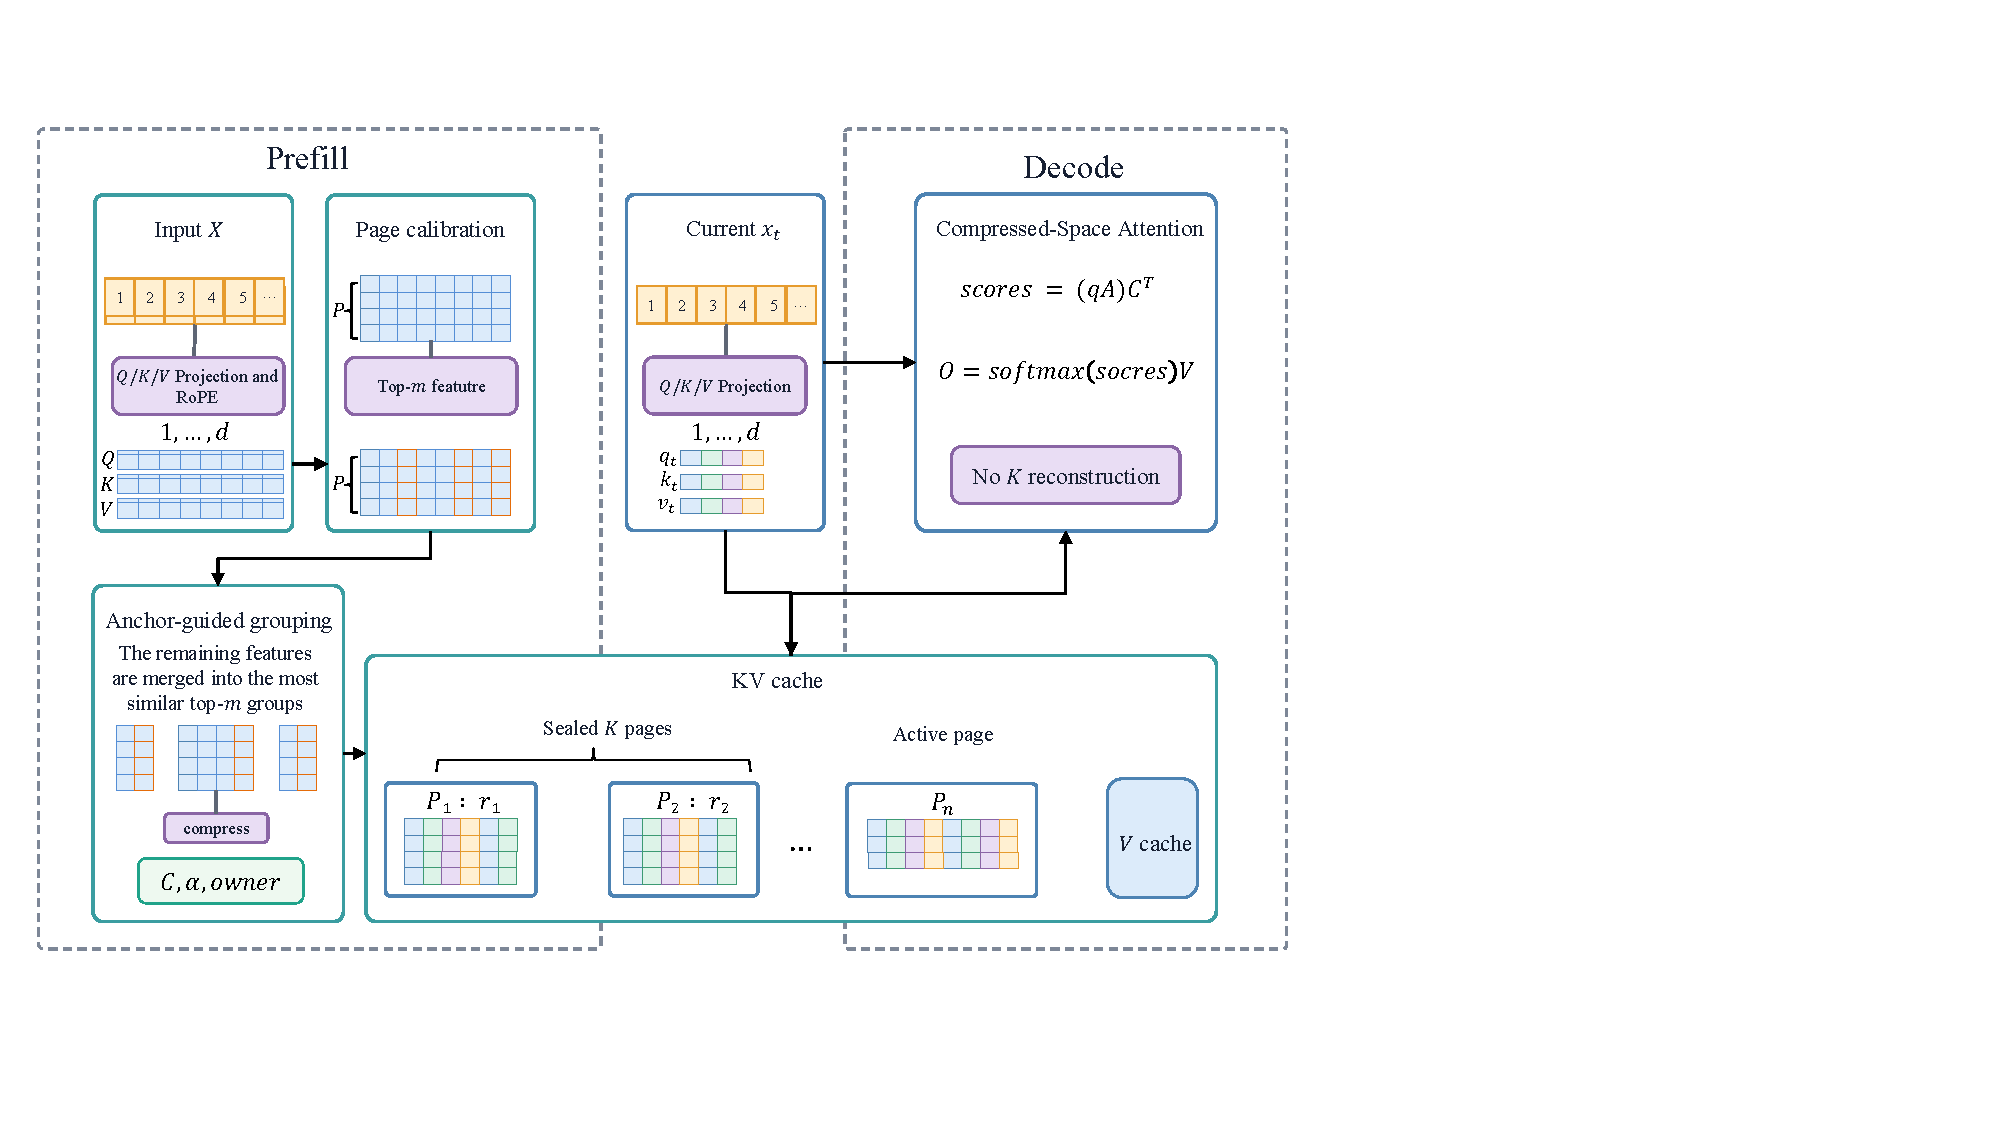
\includegraphics[width=0.82\linewidth]{cofeatsvd1.pdf}
    \end{center}
    \caption{Overview of CoFeatKV. During prefill, Q/K/V projection and RoPE produce post-RoPE key pages. For each completed page, CoFeatKV selects $m$ anchor features, assigns the remaining features to the most similar anchors, and stores page directions $C$, coefficients $\alpha$, and owner indices. During decoding, the query uses the same sparse feature-to-group mapping to compute attention in the compressed space. The active page remains dense, while sealed pages avoid key reconstruction and repeated RoPE.}
    \label{fig:overview}
\end{figure}

\subsection{Attention-Aware Feature Coalescing}

To reduce the information loss caused by the weakened low-rank structure
after RoPE, CoFeatKV compresses each completed post-RoPE key page by grouping
key feature dimensions according to their attention importance and similarity.
We first identify the most important key feature dimensions and use each of
them to initialize a separate group. The remaining feature dimensions are then
assigned to the group with the most similar key structure. This prevents
high-importance features from being merged with one another, while allowing
similar remaining features to share the same group representation.

For each KV head, we partition the post-RoPE keys along the token dimension
into fixed-size pages of $P$ tokens. Let
$K\in\mathbb{R}^{P\times d}$ denote one completed page, and let
$k_j=K_{:,j}\in\mathbb{R}^{P}$ denote feature dimension $j$ across the page.
Since the contribution of a feature to the attention score depends on both
its key representation and the corresponding query dimension, we estimate
feature importance using

\begin{equation}
    w_j=
    \frac{1}{GP}\sum_{g,t}Q_{\mathrm{page}}[g,t,j]^2,
    \qquad
    s_j=w_j\|k_j\|_2^2,
    \label{eq:importance}
\end{equation}

where $w_j$ measures the query importance of feature $j$, and $s_j$ is the
resulting importance score after combining $w_j$ with the squared $\ell_2$
norm of the corresponding key feature. A larger $s_j$ indicates a more
important feature for attention.

Given a group budget $m<d$, we select the top-$m$ features according to $s_j$
as group representatives. For each remaining feature $\ell$, we measure the
information loss caused by merging it with representative $h$. Specifically,
we consider the query-weighted pair
$\left[\sqrt{w_h}k_h,\sqrt{w_\ell}k_\ell\right]$ and use the residual error of
its best rank-one approximation as the merge cost:

\begin{equation}
\Delta(h,\ell)=
\frac{1}{2}
\left(
a_h+b_\ell-
\sqrt{(a_h-b_\ell)^2+4c_{h\ell}+\varepsilon}
\right),
\end{equation}

where
$a_h=w_h\|k_h\|_2^2$,
$b_\ell=w_\ell\|k_\ell\|_2^2$, and
$c_{h\ell}=w_hw_\ell(k_h^\top k_\ell)^2$.
A smaller $\Delta(h,\ell)$ means that the two feature dimensions can be
represented by one shared direction with less information loss. We therefore
assign

\begin{equation}
g(\ell)=\arg\min_h\Delta(h,\ell).
\end{equation}

The closed form above is the residual of the best rank-one approximation of
the weighted two-feature matrix; its derivation is given in
Appendix~\ref{app:merge-derivation}. The assignment is a greedy,
page-local criterion rather than a claim of globally optimal clustering. In
particular, $w_j$ is computed once from the queries observed while the page is
being formed; future queries do not trigger regrouping. The effect of this
calibration choice is covered by the conditional attention-error bound in
Appendix~\ref{app:error-analysis}.


\subsection{Structured Shared-Feature Representation}

To reduce the projection storage overhead of conventional low-rank methods,
CoFeatKV uses one shared group direction and one scalar coefficient for each
key feature dimension, reducing the storage required for projection
coefficients from $dm$ to $d$.

For group $r$, let $\mathcal{G}_r$ denote the set of key feature dimensions
assigned to this group:
\begin{equation}
    \mathcal{G}_r=\{j:g(j)=r\}.
\end{equation}
Then, we compute one shared direction to represent all features in
$\mathcal{G}_r$. Specifically,
\begin{equation}
    S_r=\sum_{j\in\mathcal{G}_r} w_j k_jk_j^\top,
    \qquad
    c_r=\operatorname{principal\_eigenvector}(S_r).
    \label{eq:group-direction}
\end{equation}
Here, $S_r$ summarizes the query-weighted structure of the features in group
$r$, and $c_r\in\mathbb{R}^{P}$ is their shared direction.

Although features in the same group share a similar direction, their
magnitudes along this direction can be different. Therefore we store one
scalar coefficient for each feature:
\begin{equation}
    \alpha_j=c_{g(j)}^\top k_j,
    \qquad
    \widehat K_{:,j}=\alpha_j c_{g(j)}.
    \label{eq:feature-approximation}
\end{equation}
For a fixed unit-norm group direction, $\alpha_j$ is the projection coefficient
of feature $j$ onto that direction.

Collecting the $m$ group directions gives
\begin{equation}
    C=[c_1,\ldots,c_m]\in\mathbb{R}^{P\times m}.
\end{equation}
Collecting the approximations of all key feature dimensions gives
\begin{equation}
    \widehat K=CA^\top,
    \qquad
    A_{j,r}=
    \begin{cases}
        \alpha_j, & r=g(j),\\
        0, & \text{otherwise}.
    \end{cases}
    \label{eq:sparse-projection}
\end{equation}

Since each key feature dimension belongs to one group, CoFeatKV does
not need to store the dense coefficient matrix $A$. Instead, for each page it
stores only the group directions
\begin{equation}
    C\in\mathbb{R}^{P\times m},\qquad
    \alpha\in\mathbb{R}^{d},\qquad
    \operatorname{owner}\in\{1,\ldots,m\}^{d},
\end{equation}
where $\operatorname{owner}_j=g(j)$ is the group assignment of feature
$j$, and $\alpha_j$ is its scalar coefficient. In contrast, a conventional
dense approximation stores $d\times m$ projection coefficients. CoFeatKV
reduces this to one coefficient and one group index per feature, so the number
of projection coefficients decreases from $dm$ to $d$. Correlated features
reuse the same group direction, which reduces the per-page projection storage.


\subsection{Reconstruction-Free Grouped Attention}

During decoding, reconstructing the full historical Key matrix before
attention introduces additional computation. To reduce this cost, CoFeatKV
computes attention from the grouped representation. For a post-RoPE query
$q\in\mathbb{R}^{d}$,

\begin{equation}
    q\widehat K^\top
    =
    qAC^\top
    =
    (qA)C^\top.
    \label{eq:direct-attn}
\end{equation}

Since both the query and the compressed Key representation are in the
post-RoPE space, attention can be computed as $(qA)C^\top$. The query uses
the feature groups determined by the Key page to form $qA$, which is then
multiplied by $C^\top$ to obtain the attention scores. This computation
requires neither Key reconstruction nor additional RoPE.

\begin{figure}[t]
    \begin{center}
    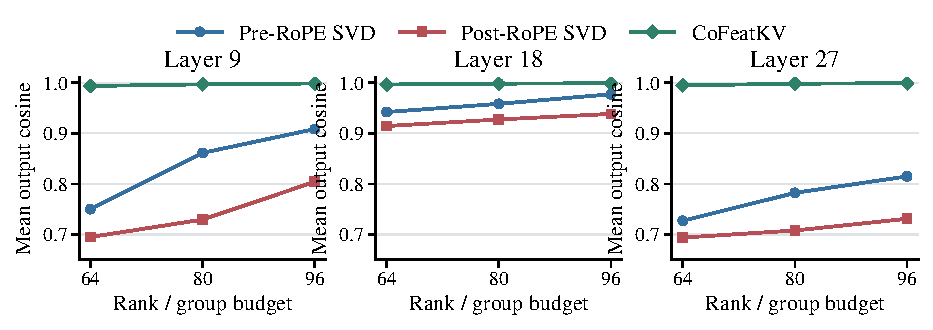
\includegraphics[width=0.82\linewidth]{figures/feature_similarity.pdf}
    \end{center}
    \caption{Layer-wise attention-output fidelity on Qwen3-8B. Each panel is
    a zero-based layer and reports mean output cosine similarity to Full.
    Values are averaged over all query heads and tokens in one 4096-token
    WikiText-2 window.}
    \label{fig:similarity}
\end{figure}

\if 0
\subsection{Paged Runtime and Storage}

CoFeatKV seals a page only after it reaches $P$ tokens. During autoregressive
decoding, the newest page remains dense so that new tokens can be appended
without refitting previous pages. When the page is full, the implementation
computes its importance scores, forms the group directions, and writes the
compact tuple $(C,\alpha,\operatorname{owner})$. The dense Key buffer for that
page can then be released; sealed pages are not regrouped later. This page
boundary makes the fitting cost local and avoids modifying the historical
cache at every decoding step.

For grouped-query attention (GQA), all query heads mapped to the same KV head
reuse the same page representation. The kernel computes $(qA)C^\top$ for each
sealed page and combines its partial statistics with the dense active page
using online softmax. The implementation keeps the score, softmax, and output
accumulation in FP32, while the stored group directions and coefficients use
the cache precision. The decode path therefore reads the compressed
representation directly and never materializes a historical Key page.

For one sealed page, the Key storage is

\begin{equation}
Pm b_C+d b_\alpha+d b_{\mathrm{owner}},
\label{eq:storage}
\end{equation}

compared with $Pd b_K$ bytes for dense Keys, where $b_C$, $b_\alpha$,
$b_{\mathrm{owner}}$, and $b_K$ denote the corresponding element sizes.
The first term stores the $m$ page-length directions. The remaining two terms
store one coefficient and one group index per feature. This is the key storage
advantage of CoFeatKV: a dense latent projection would require $dm$
coefficients, whereas the one-owner mapping requires only $d$ coefficients
and $d$ compact indices. For example, with BF16 directions and coefficients,
an 8-bit owner index, $P=32$, $d=128$, and $m=80$, a page requires 5,504
bytes for Keys before allocator alignment, compared with 8,192 bytes for a
dense BF16 page. Values are orthogonal to the Key representation and may be
quantized independently.
\fi


\begin{table}[H]
\centering
\caption{LongBench results on Meta-Llama-3.1-8B-Instruct over four question-answering
tasks. Avg. is the unweighted mean. }
\label{tab:longbench-llama}
\small
\setlength{\tabcolsep}{3.5pt}
\begin{tabular}{lrrrrr}
\toprule
Method & Qasper & MFQA & HotpotQA & 2WikiMQA & Avg. \\
\midrule
FullKV & 46.05 & 53.68 & 52.25 & 39.35 & 47.83 \\
PaLu~\citep{palu} & 29.15 & 38.61 & 25.07 & 36.41 & 32.31 \\
OjaKV~\citep{ojakv} & 35.65 & 46.77 & 38.94 & 34.28 & 38.91 \\
ReCalKV~\citep{recalkv} & 24.47 & 40.25 & 8.82 & 6.22 & 19.94 \\
CoFeatKV ($m=80$) &45.76 & 54.29 & 52.25 & 42.68 & 48.75 \\
\bottomrule
\end{tabular}
\end{table}
\section{Experiments}
\label{sec:experiments}

\subsection{Experimental setup}

\paragraph{Models and benchmarks.}
Our experiments use Meta-Llama-3.1-8B-Instruct (Dubey et al., 2024),
Qwen3-8B, Qwen3-32B, and Llama-2-7B. We evaluate on LongBench
(Bai et al., 2023), RULER (Hsieh et al., 2024), MMLU (Hendrycks et al.,
2021), and WikiText-2 (Merity et al., 2017).

\paragraph{Baselines.}
We use FullKV with the original KV cache as the uncompressed reference.
We compare CoFeatKV with four low-rank KV-cache compression methods covering
different designs: PaLu~\citep{palu} performs offline factorization
of projection weights, ReCalKV~\citep{recalkv} determines ranks using
calibration data, OjaKV~\citep{ojakv} updates the low-rank subspace
during inference, and PuzzleKV~\citep{puzzlekv} applies decomposition
at the page level. For methods with released implementations, we run the
baselines in our local evaluation environment.

\if 0
\paragraph{Metrics.}
We report perplexity (PPL), mean attention-output cosine similarity, relative
squared output error
$\|O-O_{\mathrm{Full}}\|_F^2/\|O_{\mathrm{Full}}\|_F^2$, weighted page-wise
Key approximation error, factor-to-dense storage ratio, and decode throughput.
For RULER, we report task accuracy and the unweighted macro-average across
tasks. For LongBench, we use the official metric for each task and report the
unweighted average. We compute cosine similarity and output error over all
query heads and tokens in the selected WikiText-2 window.
\paragraph{Runtime and storage configuration.}
The Qwen3-8B controlled experiments run on one GPU. Qwen3-32B RULER runs shard
the model across four GPUs, while each Llama-3.1-8B RULER worker uses one GPU.
All generation runs use batch size one, greedy decoding, BF16 model states,
and seed 42. Score, softmax, output, and metric reductions use FP32. Runtime
measurements report decode tokens per second and process-level CUDA
allocation; the latter includes model weights and temporary workspace.
\fi
\paragraph{CoFeatKV configuration.}
Runtime and attention-output experiments use 32-token pages. The page-local
representation study uses 128-token pages to expose the effect of the group
budget. Unless stated otherwise, we test $m\in\{64,80,96\}$. %Group directions
%and feature coefficients use BF16, owner indices use 8-bit integers, and the
%active page remains dense. The Qwen3-8B and Llama-3.1-8B long-context runs use
%$m=80$; the reported Qwen3-32B pilot uses $m=64$.


\if 0
\begin{figure}[t]
    \begin{center}
    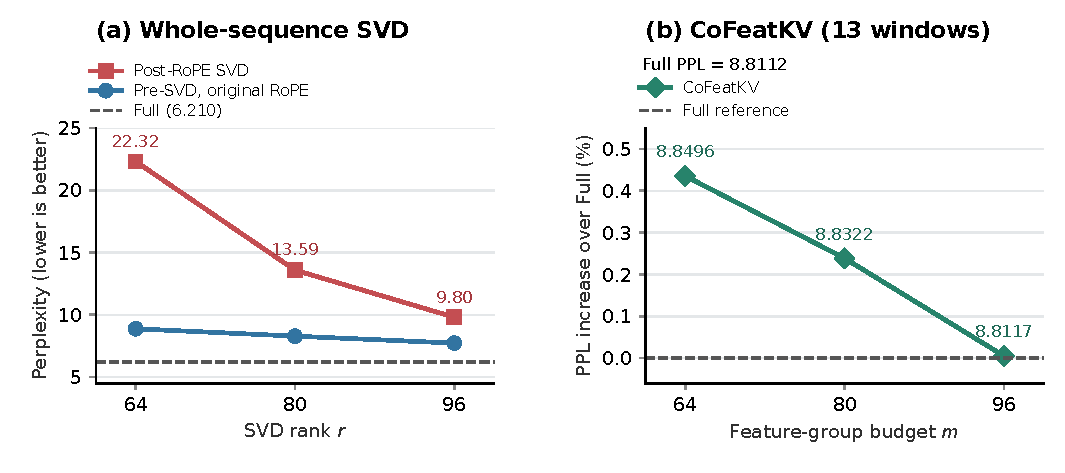
\includegraphics[width=0.93\linewidth]{figures/rope_same_rank.pdf}
    \end{center}
    \caption{Two complementary Qwen3-8B diagnostics. (a) Whole-sequence SVD
    compares pre-RoPE and post-RoPE compression at the same rank on one
    4096-token window. (b) Page-wise CoFeatKV evaluation across 13 windows.
    The two panels use different protocols and are not a single pooled
    benchmark.}
    \label{fig:rope}
\end{figure}
Figure~\ref{fig:rope}(a) isolates the effect of applying SVD after RoPE. At
$r=64$, pre-RoPE SVD obtains PPL 8.87, while post-RoPE SVD reaches 22.32.
The gap narrows as the rank grows, but post-RoPE SVD remains worse at $r=80$
(13.59 versus 8.28) and $r=96$ (9.80 versus 7.72). RoPE therefore makes one
shared basis less effective. CoFeatKV keeps the post-RoPE representation and
uses page-local feature sharing to recover the lost accuracy.

Figure~\ref{fig:rope}(b) reports the 13-window CoFeatKV PPL study. The Full
reference is 8.8112. CoFeatKV obtains 8.8496, 8.8322, and 8.8117 for
$m=64,80,96$, which increases PPL by 0.435\%, 0.239\%, and 0.005\%.
Increasing $m$ recovers the dense-cache PPL. The two panels use different
sequence protocols: the left panel uses one 4096-token window, whereas the
right panel aggregates 13 windows.

\begin{table}[H]
    \centering
    \caption{Whole-sequence SVD results on one 4096-token WikiText-2 window.
    Discarded energy measures the fraction removed by the truncated factorization.}
    \label{tab:rope-ppl}
    \small
    \setlength{\tabcolsep}{3.5pt}
    \begin{tabular}{lccc|ccc}
        \toprule
        Method & \multicolumn{3}{c|}{PPL} & \multicolumn{3}{c}{Discarded energy} \\
        & $r=64$ & $r=80$ & $r=96$ & $r=64$ & $r=80$ & $r=96$ \\
        \midrule
        Full & 6.2103 & -- & -- & -- & -- & -- \\
        Pre-RoPE SVD  & 8.8739 & 8.2832 & 7.7226 & 0.0152 & 0.0080 & 0.0032 \\
        Post-RoPE SVD & 22.3186 & 13.5907 & 9.7994 & 0.0502 & 0.0310 & 0.0169 \\
        \bottomrule
    \end{tabular}
\end{table}


\subsection{Layer-wise attention-output fidelity}



Figure~\ref{fig:similarity} gives a direct test of the quantity that the
compressed attention kernel consumes. At $m=80$, CoFeatKV obtains cosine
similarities 0.9969, 0.9982, and 0.9981 at layers 9, 18, and 27. Pre-RoPE SVD
obtains 0.8614, 0.9584, and 0.7823, while post-RoPE SVD obtains 0.7295, 0.9274,
and 0.7078. Table~\ref{tab:layer-error} reports the corresponding relative
squared errors. At layer 27, the error of post-RoPE SVD reaches 2.2266 at
$r=80$, while CoFeatKV remains at 0.0047. Grouping therefore preserves the
attention output at the layer where a single post-RoPE basis loses the most
information.

\begin{table}[H]
\centering
\caption{Relative squared attention-output error on the same captured
Qwen3-8B sequence. Lower is better.}
\label{tab:layer-error}
\small
\setlength{\tabcolsep}{4pt}
\begin{tabular}{lrrrr}
\toprule
Budget & Layer 9 & Layer 18 & Layer 27 & Mean \\
\midrule
Pre-RoPE SVD-64  & 0.4669 & 0.1207 & 2.0773 & 0.8883 \\
Post-RoPE SVD-64 & 0.5574 & 0.1744 & 2.2541 & 0.9953 \\
CoFeatKV-$m=64$  & 0.0150 & 0.0071 & 0.0140 & 0.0121 \\
Pre-RoPE SVD-80  & 0.3247 & 0.0799 & 1.7441 & 0.7162 \\
Post-RoPE SVD-80 & 0.4918 & 0.1438 & 2.2266 & 0.9541 \\
CoFeatKV-$m=80$  & 0.0071 & 0.0036 & 0.0047 & 0.0051 \\
Pre-RoPE SVD-96  & 0.2675 & 0.0431 & 1.4517 & 0.5874 \\
Post-RoPE SVD-96 & 0.4138 & 0.1183 & 2.0674 & 0.8665 \\
CoFeatKV-$m=96$  & 0.0030 & 0.0017 & 0.0016 & 0.0021 \\
\bottomrule
\end{tabular}
\end{table}

\begin{table}[H]
\centering
\caption{Mean cosine similarity between each method and Full attention,
measured before $o_{\mathrm{proj}}$. Higher is better.}
\label{tab:layer-cosine}
\small
\setlength{\tabcolsep}{4pt}
\begin{tabular}{lrrrr}
\toprule
Budget & Layer 9 & Layer 18 & Layer 27 & Mean \\
\midrule
Pre-RoPE SVD-64  & 0.7502 & 0.9421 & 0.7271 & 0.8065 \\
Post-RoPE SVD-64 & 0.6949 & 0.9144 & 0.6940 & 0.7678 \\
CoFeatKV-$m=64$  & 0.9937 & 0.9966 & 0.9950 & 0.9951 \\
Pre-RoPE SVD-80  & 0.8614 & 0.9584 & 0.7823 & 0.8674 \\
Post-RoPE SVD-80 & 0.7295 & 0.9274 & 0.7078 & 0.7883 \\
CoFeatKV-$m=80$  & 0.9969 & 0.9982 & 0.9981 & 0.9977 \\
Pre-RoPE SVD-96  & 0.9085 & 0.9773 & 0.8149 & 0.9003 \\
Post-RoPE SVD-96 & 0.8042 & 0.9385 & 0.7311 & 0.8246 \\
CoFeatKV-$m=96$  & 0.9986 & 0.9992 & 0.9993 & 0.9990 \\
\bottomrule
\end{tabular}
\end{table}

At $m=64$, CoFeatKV reaches mean cosine 0.9951, compared with 0.8065 for
pre-RoPE SVD and 0.7678 for post-RoPE SVD. The mean relative squared errors
are 0.0121, 0.8883, and 0.9953, respectively. The late layer 27 shows the
same pattern: CoFeatKV reaches cosine 0.9950, while pre-RoPE and post-RoPE
SVD reach 0.7271 and 0.6940.
\fi

\if 0
\subsection{Page-local grouping and representation capacity}

The 32-sequence page diagnostic provides a second view of the grouping rule.
With page size 128 and $m=80$, the mean weighted Key approximation error is
0.0665, 0.0479, and 0.0566 at layers 9, 18, and 27. The corresponding mean
ranks needed to retain 95\% of page energy are 36.3, 34.2, and 34.8, which is
well below the tested group budget. This supports the use of page-local shared
directions rather than a single global basis.

\begin{table}[H]
\centering
\caption{Effective ranks of pre-RoPE and post-RoPE Key matrices. Each entry
denotes the rank that retains the indicated fraction of spectral energy.}
\label{tab:effective-rank}
\small
\setlength{\tabcolsep}{5pt}
\begin{tabular}{rcccccc}
\toprule
Layer & \multicolumn{2}{c}{$r_{90}$} & \multicolumn{2}{c}{$r_{95}$} & \multicolumn{2}{c}{$r_{99}$} \\
 & Pre & Post & Pre & Post & Pre & Post \\
\midrule
9  & 17.8 & 24.7 & 28.7 & 37.7 & 55.5 & 66.8 \\
18 & 13.4 & 17.9 & 23.3 & 30.8 & 50.1 & 61.6 \\
27 & 14.5 & 20.6 & 25.7 & 33.7 & 53.8 & 63.6 \\
\bottomrule
\end{tabular}
\end{table}

\begin{table}[H]
\centering
\caption{Page-local CoFeatKV statistics for 32 WikiText-2 sequences with
page size 128 and $m=80$.}
\label{tab:group-summary}
\small
\setlength{\tabcolsep}{6pt}
\begin{tabular}{rccc}
\toprule
Layer & Weighted Key error & $r_{95}$ & $r_{99}$ \\
\midrule
9  & 0.0665 & 36.3 & 54.9 \\
18 & 0.0479 & 34.2 & 53.9 \\
27 & 0.0566 & 34.8 & 54.2 \\
\bottomrule
\end{tabular}
\end{table}

\begin{table}[H]
\centering
\caption{Mean weighted Key approximation error over 32 WikiText-2
sequences, using page size 128. Increasing the group budget reduces the error
at all three inspected layers, with diminishing returns after $m=64$.}
\label{tab:group-error}
\small
\setlength{\tabcolsep}{5pt}
\begin{tabular}{rccc}
\toprule
$m$ & Layer 9 & Layer 18 & Layer 27 \\
\midrule
8  & 0.3258 & 0.2287 & 0.2518 \\
16 & 0.2185 & 0.1525 & 0.1695 \\
24 & 0.1567 & 0.1136 & 0.1250 \\
32 & 0.1196 & 0.0900 & 0.0989 \\
48 & 0.0833 & 0.0643 & 0.0718 \\
64 & 0.0703 & 0.0525 & 0.0605 \\
80 & 0.0665 & 0.0479 & 0.0566 \\
\bottomrule
\end{tabular}
\end{table}

\begin{figure}[ht]
    \begin{center}
    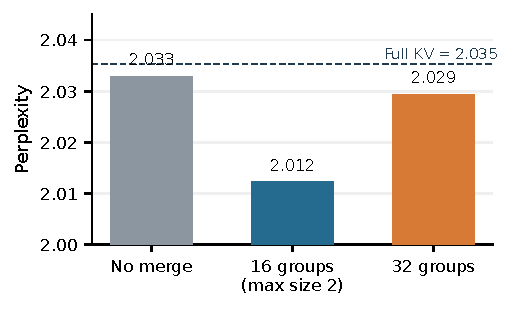
\includegraphics[width=0.68\linewidth]{figures/group_ablation.pdf}
    \end{center}
    \caption{Grouping ablation in a short end-to-end Qwen3-8B run. The
    16-group configuration gives the lowest PPL among the tested variants.}
    \label{fig:ablation}
\end{figure}

The short ablation in Figure~\ref{fig:ablation} compares the same fused path
with different grouping choices. Full attention gives PPL 2.035. Removing the
merge operation gives 2.033, while 16 groups with maximum group size two gives
2.012 and 32 groups gives 2.029. The lowest PPL does not occur at the largest
group count. The grouping rule allocates capacity using feature similarity and
attention importance, rather than only increasing the number of coordinates.

\begin{table}[H]
\centering
\caption{Grouping ablation on the same short Qwen3-8B run. Factor / dense
reports stored factor bytes divided by dense FP16 KV bytes.}
\label{tab:group-ablation}
\small
\setlength{\tabcolsep}{4pt}
\begin{tabular}{lrrr}
\toprule
Grouping variant & PPL & Factor / dense & Fit blocks \\
\midrule
No merge & 2.0330 & 0.8292 & 960 \\
16 groups, max size 2 & 2.0123 & 0.7429 & 960 \\
32 groups & 2.0294 & 0.7212 & 960 \\
\bottomrule
\end{tabular}
\end{table}

\subsection{End-to-end direct execution}

We next run the complete autoregressive path. In the matched Qwen3-8B
experiment, the input contains 128 prefill tokens and the evaluation decodes
2,048 tokens. The run records PPL, decode throughput, process-level CUDA
allocation, and Key reconstruction calls.

\begin{table}[H]
\centering
\caption{Matched Qwen3-8B quality and runtime run with 128 prefill tokens
and 2,048 decode tokens. Peak allocation is the process-level CUDA
allocation, not an isolated KV-cache measurement.}
\label{tab:end-to-end-matched}
\small
\setlength{\tabcolsep}{4pt}
\begin{tabular}{lrrrr}
\toprule
Method & PPL & Decode tok/s & Peak allocated (GB) & K recon. calls \\
\midrule
Full & 5.9339 & 26.51 & 16.7602 & -- \\
CoFeatKV-$m=80$ & 5.9593 & 29.62 & 17.0025 & 0 \\
\bottomrule
\end{tabular}
\end{table}

CoFeatKV changes PPL from 5.9339 to 5.9593 and increases decode throughput
from 26.51 to 29.62 tokens/s. The run records zero Key reconstruction calls.
The process-level allocation changes from 16.7602 to 17.0025 GB because the
measurement includes model weights and temporary workspace. It does not equal
the persistent KV-cache size. A separate 2,176-token run reaches PPL 5.9593,
36.54 tokens/s, and zero Key reconstruction calls, which confirms the direct
path at a longer sequence.

In a 30-layer fused storage run, CoFeatKV stores 25.77 MB of factors for a
62.91 MB dense FP16 KV representation, giving a factor-to-dense ratio of
0.410. The compressed run obtains PPL 6.2082, compared with 6.2433 for Full.
This result measures representation storage; the page-fitting cost remains a
separate systems cost.

\begin{table}[H]
\centering
\caption{Storage comparison in the 30-layer fused run. The table reports
factor storage and does not include transient page-fitting workspace.}
\label{tab:storage}
\small
\setlength{\tabcolsep}{8pt}
\begin{tabular}{lrr}
\toprule
Representation & Stored bytes (MB) & Relative to dense \\
\midrule
Dense FP16 KV & 62.91 & 1.000 \\
CoFeatKV factors & 25.77 & 0.410 \\
\bottomrule
\end{tabular}
\end{table}
\fi





\if 0
\paragraph{Qwen model coverage and generation audit.}
Tables~\ref{tab:longbench-qwen8b-audit} and~\ref{tab:longbench-qwen32b-audit}
report scores of the available Qwen predictions without post-processing.
These are generation diagnostics, not validated compression-quality results.
In Qwen3-8B, all 200 HotpotQA outputs from both FullKV and CoFeatKV contain
an opening \texttt{<think>} tag but no closing tag. The generation budget
therefore expires before the reasoning segment finishes. This affects the
uncompressed reference as well as our method. The direct FullKV and CoFeatKV
loops also omit end-of-sequence stopping checks. Correct stopping rules and
an explicit reasoning-mode policy are required before rerunning the evaluation.
We report partial-task scores with their sample counts and omit full-suite
averages. We do not rank methods using these diagnostic runs.

\begin{table}[H]
\centering
\caption{Qwen3-8B LongBench raw-run diagnostics, pending correction
of generation settings. Superscripts $[n]$ mark partial tasks with $n$
scored predictions. Unmarked scores use 200 examples, except MFQA (150)
and RepoBench-P (500). A dash denotes an unavailable score; no complete-suite
average is reported.}
\label{tab:longbench-qwen8b-audit}
\small
\setlength{\tabcolsep}{3pt}
\begin{tabular}{lrrrr}
\toprule
Method & Qasper & MFQA & HotpotQA & 2WikiMQA \\
\midrule
FullKV & 12.00 & 14.11 & 2.84 & 7.54 \\
PaLu~\citep{palu} & 9.01 & 16.15 & 4.95 & 7.35 \\
OjaKV~\citep{ojakv} & 7.10$^{[57]}$ & 14.05 & 2.79 & 7.65 \\
ReCalKV~\citep{recalkv} & 9.15 & 13.60 & 2.47 & 6.53 \\
CoFeatKV ($m=64$) & -- & -- & -- & -- \\
CoFeatKV ($m=80$) & 11.89 & 13.74 & 2.91 & 7.68 \\
\bottomrule
\end{tabular}
\par\medskip
\begin{tabular}{lrrrrr}
\toprule
Method & GovReport & QMSum & TREC & RepoBench-P & Avg. \\
\midrule
FullKV & 28.32$^{[56]}$ & 17.52 & 71.50 & 62.87$^{[224]}$ & -- \\
PaLu~\citep{palu} & 28.42$^{[56]}$ & 18.16 & 69.00 & 46.02$^{[224]}$ & -- \\
OjaKV~\citep{ojakv} & 20.63$^{[29]}$ & 16.85$^{[19]}$ & 70.50 & 37.03$^{[34]}$ & -- \\
ReCalKV~\citep{recalkv} & 27.66$^{[56]}$ & 18.02 & 70.00 & 41.79$^{[224]}$ & -- \\
CoFeatKV ($m=64$) & -- & -- & -- & -- & -- \\
CoFeatKV ($m=80$) & 27.90$^{[56]}$ & 17.33 & 72.00 & 61.91$^{[224]}$ & -- \\
\bottomrule
\end{tabular}
\end{table}

\begin{table}[H]
\centering
\caption{Qwen3-32B LongBench raw-run diagnostics, pending correction
of generation settings. Superscripts $[n]$ mark partial tasks with $n$
scored predictions. Unmarked scores use 200 examples, except MFQA (150)
and RepoBench-P (500). A dash denotes an unavailable score; no complete-suite
average is reported. The CoFeatKV runs contain only one-example Qasper smoke tests, which are excluded.}
\label{tab:longbench-qwen32b-audit}
\small
\setlength{\tabcolsep}{3pt}
\begin{tabular}{lrrrr}
\toprule
Method & Qasper & MFQA & HotpotQA & 2WikiMQA \\
\midrule
FullKV & 12.05 & 14.95 & 2.94 & 7.74 \\
CoFeatKV ($m=64$) & -- & -- & -- & -- \\
CoFeatKV ($m=80$) & -- & -- & -- & -- \\
\bottomrule
\end{tabular}
\par\medskip
\begin{tabular}{lrrrrr}
\toprule
Method & GovReport & QMSum & TREC & RepoBench-P & Avg. \\
\midrule
FullKV & 29.49$^{[56]}$ & -- & -- & -- & -- \\
CoFeatKV ($m=64$) & -- & -- & -- & -- & -- \\
CoFeatKV ($m=80$) & -- & -- & -- & -- & -- \\
\bottomrule
\end{tabular}
\end{table}

The separate Qwen3-8B ten-example-per-task pilot is not pooled with these
larger runs. For Qwen3-32B, FullKV has 806 saved predictions; CoFeatKV has only
one-example Qasper smoke tests at each of $m=64$ and $m=80$, not a formal
benchmark evaluation.
\fi



\begin{table}[H]
\centering
\caption{RULER results on Llama-3.1-8B-Instruct and Qwen3-8B at 16K and 32K context lengths.}
\label{tab:ruler-matched}
\small
\setlength{\tabcolsep}{1.2pt}
\begin{tabular}{@{}cclrrrrrrrr@{}}
\toprule
Model & Length & Method & S1 & S2 & S3 & MK1 & MK2 & MV & MQ & Avg. \\
\midrule
\multirow{7}{*}{\shortstack{Llama-3.1-8B\\Instruct}} & \multirow{7}{*}{16K} & FullKV & 100.00 & 100.00 & 100.00 & 99.00 & 100.00 & 99.50 & 99.25 & 99.68 \\
\cmidrule(lr){3-11}
 & & PaLu~\citep{palu} & \textbf{100.00} & 99.00 & \textbf{100.00} & 98.00 & 95.00 & 96.25 & 96.50 & 97.82 \\
 & & OjaKV~\citep{ojakv} & 97.00 & \textbf{100.00} & 98.00 & 97.00 & 41.00 & 97.75 & 84.25 & 87.86 \\
 & & ReCalKV~\citep{recalkv} & \textbf{100.00} & \textbf{100.00} & \textbf{100.00} & 95.00 & 99.00 & 94.00 & 96.50 & 97.79 \\
 & & PuzzleKV~\citep{puzzlekv} & 98.80 & 95.80 & 82.00 & 98.20 & \textbf{100.00} & 91.10 & 98.85 & 94.96 \\
 & & CoFeatKV ($m=64$) & \textbf{100.00} & \textbf{100.00} & \textbf{100.00} & 99.20 & \textbf{100.00} & \textbf{98.05} & 99.85 & 99.59 \\
 & & CoFeatKV ($m=80$) & \textbf{100.00} & \textbf{100.00} & \textbf{100.00} & \textbf{100.00} & 99.80 & 97.90 & \textbf{99.95} & \textbf{99.66} \\
\midrule
\multirow{7}{*}{\shortstack{Llama-3.1-8B\\Instruct}} & \multirow{7}{*}{32K} & FullKV & 100.00 & 100.00 & 99.00 & 97.00 & 100.00 & 99.50 & 99.75 & 99.32 \\
\cmidrule(lr){3-11}
 & & PaLu~\citep{palu} & \textbf{100.00} & \textbf{100.00} & 99.00 & 97.00 & 97.00 & 95.50 & 97.00 & 97.93 \\
 & & OjaKV~\citep{ojakv} & \textbf{100.00} & 99.00 & 98.00 & 94.00 & 24.00 & 97.50 & 94.25 & 86.68 \\
 & & ReCalKV~\citep{recalkv} & \textbf{100.00} & \textbf{100.00} & 96.00 & 96.00 & 96.00 & 87.25 & 95.25 & 95.79 \\
 & & PuzzleKV~\citep{puzzlekv} & 99.80 & 97.60 & 83.00 & 96.60 & 99.80 & 91.40 & 98.85 & 95.29 \\
 & & CoFeatKV ($m=64$) & \textbf{100.00} & \textbf{100.00} & \textbf{100.00} & 99.00 & \textbf{100.00} & \textbf{99.25} & \textbf{99.75} & 99.71 \\
 & & CoFeatKV ($m=80$) & \textbf{100.00} & \textbf{100.00} & \textbf{100.00} & \textbf{99.80} & 99.80 & 99.15 & 99.70 & \textbf{99.78} \\
\midrule
\multirow{7}{*}{Qwen3-8B} & \multirow{7}{*}{16K} & FullKV & 100.00 & 100.00 & 100.00 & 100.00 & 100.00 & 99.25 & 99.25 & 99.79 \\
\cmidrule(lr){3-11}
 & & PaLu~\citep{palu} & \textbf{100.00} & 98.00 & 99.00 & 98.00 & 96.00 & 96.00 & 92.25 & 97.04 \\
 & & OjaKV~\citep{ojakv} & 84.00 & 81.00 & 60.00 & 89.00 & 60.00 & 32.75 & 69.25 & 68.00 \\
 & & ReCalKV~\citep{recalkv} & \textbf{100.00} & \textbf{100.00} & \textbf{100.00} & \textbf{100.00} & 92.00 & 87.25 & 69.00 & 92.61 \\
 & & PuzzleKV~\citep{puzzlekv} & \textbf{100.00} & \textbf{100.00} & 99.00 & 99.60 & \textbf{99.80} & \textbf{99.90} & \textbf{99.90} & 99.74 \\
 & & CoFeatKV ($m=64$) & \textbf{100.00} & \textbf{100.00} & \textbf{100.00} & \textbf{100.00} & 99.59 & 99.65 & 99.83 & 99.87 \\
 & & CoFeatKV ($m=80$) & \textbf{100.00} & \textbf{100.00} & \textbf{100.00} & \textbf{100.00} & 99.60 & 99.70 & 99.85 & \textbf{99.88} \\
\midrule
\multirow{7}{*}{Qwen3-8B} & \multirow{7}{*}{32K} & FullKV & 100.00 & 100.00 & 100.00 & 99.00 & 99.00 & 97.50 & 99.50 & 99.29 \\
\cmidrule(lr){3-11}
 & & PaLu~\citep{palu} & \textbf{100.00} & 98.00 & 99.00 & 99.00 & 59.00 & 90.00 & 98.25 & 91.89 \\
 & & OjaKV~\citep{ojakv} & 78.00 & 66.00 & 55.00 & 70.00 & 28.00 & 34.75 & 56.25 & 55.43 \\
 & & ReCalKV~\citep{recalkv} & \textbf{100.00} & 99.00 & \textbf{100.00} & 98.00 & 85.00 & 95.75 & 93.00 & 95.82 \\
 & & PuzzleKV~\citep{puzzlekv} & \textbf{100.00} & 99.80 & 98.60 & \textbf{99.80} & 97.00 & 98.35 & 99.60 & 99.02 \\
 & & CoFeatKV ($m=64$) & \textbf{100.00} & \textbf{100.00} & \textbf{100.00} & 99.20 & 96.80 & 99.55 & 99.60 & 99.31 \\
 & & CoFeatKV ($m=80$) & \textbf{100.00} & \textbf{100.00} & \textbf{100.00} & 99.60 & \textbf{97.60} & \textbf{99.75} & \textbf{99.75} & \textbf{99.53} \\
\bottomrule
\end{tabular}
\end{table}
\subsection{Compression before and after RoPE}


Figure~\ref{fig:similarity} shows the mean cosine similarity between the attention outputs
produced by compressed keys and those produced by the original keys. As the
rank or group budget increases from 64 to 96, both pre-RoPE SVD and post-RoPE
SVD improve, while post-RoPE SVD remains lower than pre-RoPE SVD. In contrast,
CoFeatKV maintains cosine similarity close to 1.0 across all three layers and
all tested budgets. This shows that CoFeatKV preserves more attention-relevant
information when compressing post-RoPE keys and keeps the resulting attention
outputs close to those of the original keys.

\subsection{LONG-CONTEXT Comparison on 8B Models}

We next evaluate long-context understanding on Meta-Llama-3.1-8B-Instruct using four LongBench question-answering tasks. The table reports
the official LongBench task metrics, with FullKV and baseline methods evaluated
on the same models for comparison.

As shown in Table~\ref{tab:longbench-llama}, we compare CoFeatKV with FullKV
and three low-rank baselines on four LongBench tasks. CoFeatKV achieves the
highest average score of 48.75, compared with 47.83 for FullKV. It improves
 MFQA, and 2WikiMQA, and matches FullKV on HotpotQA. Compared with the
low-rank baselines, CoFeatKV preserves important key features and shares
representations only among similar features, reducing the information loss of
post-RoPE compression. CoFeatKV exceeds FullKV on several tasks
because compression changes attention scores and can lead to different
generations; since LongBench measures task-level answer quality rather than
agreement with FullKV, some of these changes receive higher scores.

Table~\ref{tab:ruler-matched} compares CoFeatKV with FullKV and four low-rank
baselines on Llama-3.1-8B-Instruct and Qwen3-8B at 16K and 32K context
lengths. CoFeatKV matches FullKV across both models and context lengths. With
$m=80$, it reaches 99.66 and 99.78 on Llama-3.1-8B-Instruct, compared with
99.68 and 99.32 for FullKV. On Qwen3-8B, CoFeatKV achieves 99.88 and 99.53,
compared with 99.79 and 99.29 for FullKV. It also outperforms the other
compressed methods in all four settings. These results show that CoFeatKV
preserves long-context performance under post-RoPE key compression.

\subsection{Qwen3-32B Long-Context Evaluation}

we evaluate CoFeatKV on Qwen3-32B to test whether the compressed
representation remains effective at a larger model scale and longer context.
Since the baseline methods do not report results on 32B models, we compare
CoFeatKV with the standard FullKV setting on RULER. We use the first 100
examples from each of 11 tasks and evaluate both 16K and 32K context lengths
using task accuracy.

\begin{table}[H]
\centering
\caption{Per-task Qwen3-32B RULER accuracy. S1--S3 achieve 100.0 in all settings and are included in the average.}
\label{tab:ruler32b-tasks}
\scriptsize
\setlength{\tabcolsep}{3.2pt}

\resizebox{\textwidth}{!}{
\begin{tabular}{llrrrrrrrrr}
\toprule
Context & Method
& NIAH-MK1 & NIAH-MK2 & NIAH-MV & NIAH-MQ
& VT & CWE & FWE & QA-1 & Avg. \\
\midrule

16K & Full
& 100.0 & 100.0 & 100.0 & 100.0
& 100.0 & 49.30 & 91.00 & 86.00 & 93.30 \\

16K & $m=64$
& 100.0 & 100.0 & 100.0 & 100.0
& 100.0 & 71.30 & 92.00 & 84.00 & 95.21 \\

16K & $m=80$
& 100.0 & 100.0 & 100.0 & 100.0
& 100.0 & 63.20 & 92.33 & 86.00 & 94.68 \\

\midrule

32K & Full
& 100.0 & 100.0 & 100.0 & 100.0
& 100.0 & 51.90 & 92.67 & 82.00 & 93.32 \\

32K & $m=64$
& 100.0 & 100.0 & 100.0 & 100.0
& 100.0 & 60.50 & 85.00 & 81.00 & 93.32 \\

32K & $m=80$
& 100.0 & 100.0 & 100.0 & 100.0
& 100.0 & 58.00 & 91.67 & 85.00 & 94.06 \\

\bottomrule
\end{tabular}
}

\end{table}

Table~\ref{tab:ruler32b-tasks} reports the RULER results on Qwen3-32B.
CoFeatKV preserves 100\% accuracy on all NIAH tasks and VT at both 16K and
32K context lengths. At 16K, $m=64$ achieves an average score of 95.21,
compared with 93.30 for FullKV, with the largest improvement on CWE. At 32K,
$m=80$ reaches 94.06, compared with 93.32 for FullKV, while improving CWE and
QA-1. The variation mainly comes from CWE, FWE, and QA-1, whereas the retrieval
tasks remain unchanged. These results show that CoFeatKV maintains
long-context performance when scaling from 8B to Qwen3-32B.

\subsection{Ablation studies}

We examine how feature merging changes storage and prediction quality,
and how the group budget affects Key approximation, perplexity, and decode
throughput. The short end-to-end grouping study, the page-local budget sweep,
and the archived runtime comparison use different settings and are reported
separately.
\if 0
\subsubsection{Effect of feature merging.}
We compare three grouping configurations in an earlier Qwen3-8B fused
prototype: no merging, 16 groups with at most two features per group, and
32 groups. Each run uses 128 prefill tokens and 126 decode tokens.
Table~\ref{tab:ablation-merging} reports perplexity and stored factor bytes
relative to dense FP16 KV bytes. All configurations fit 960 blocks.
These prototype group counts are not the feature-anchor budget $m$
used in the next experiment.

\begin{table}[H]
\centering
\caption{Feature-merging ablation in the short Qwen3-8B prototype run.
Lower is better for both metrics. Storage counts factors, not peak GPU
memory. Bold marks the best compressed configuration in each column.}
\label{tab:ablation-merging}
\small
\setlength{\tabcolsep}{8pt}
\begin{tabular}{lrr}
\toprule
Configuration & PPL & Factor / dense KV \\
\midrule
FullKV & 2.0353 & 1.0000 \\
\midrule
No merging & 2.0330 & 0.8292 \\
16 groups, maximum size 2 & \textbf{2.0123} & 0.7429 \\
32 groups & 2.0294 & \textbf{0.7212} \\
\bottomrule
\end{tabular}
\end{table}

Merging reduces factor storage relative to the no-merge configuration.
The 16-group setting obtains the lowest PPL, whereas the 32-group setting
uses the least storage. Thus, the two objectives select different
configurations in this run. These short-sequence results do not establish
a general accuracy improvement over FullKV or a storage-matched advantage
for the current implementation.
\fi

\subsubsection{Effect of the group budget.}
We vary $m$ from 8 to 80 on 32 WikiText-2 sequences in the Qwen3-8B page
diagnostic, with 128 tokens per page. We measure weighted Key approximation
error at layers 9, 18, and 27, using zero-based layer indices.
This metric measures Key reconstruction under the compression objective,
not task accuracy or attention-output error.

\begin{table}[H]
\centering
\caption{Group-budget sensitivity of weighted Key approximation error.
Results average over 32 WikiText-2 sequences with page size 128.
Lower is better; bold marks the smallest error in each layer.}
\label{tab:ablation-budget}
\small
\setlength{\tabcolsep}{9pt}
\begin{tabular}{rrrr}
\toprule
$m$ & Layer 9 & Layer 18 & Layer 27 \\
\midrule
8  & 0.3258 & 0.2287 & 0.2518 \\
16 & 0.2185 & 0.1525 & 0.1695 \\
24 & 0.1567 & 0.1136 & 0.1250 \\
32 & 0.1196 & 0.0900 & 0.0989 \\
48 & 0.0833 & 0.0643 & 0.0718 \\
64 & 0.0703 & 0.0525 & 0.0605 \\
80 & \textbf{0.0665} & \textbf{0.0479} & \textbf{0.0566} \\
\bottomrule
\end{tabular}
\end{table}

As shown in Table~\ref{tab:ablation-budget}, increasing $m$ consistently reduces
the approximation error across all three layers, with smaller gains at larger
budgets. In Layer 9, increasing $m$ from 32 to 64 reduces the error from
0.1196 to 0.0703, while increasing $m$ from 64 to 80 further reduces it to
0.0665. Layers 18 and 27 show the same trend. 

\subsubsection{Effect of Group Budget on Compression, Throughput, and Quality}
We evaluate Qwen3-8B results on WikiText-2 with
$m\in\{64,80,96\}$ to measure how the group budget affects KV-cache
compression, decoding throughput, and model quality. All runs use BF16 on a
single RTX 3090 with batch size 1, a 128-token prefill, followed by 2048
autoregressive decoding steps.

% Sources: /home/jhl_1/llm_inter/pukkz_svd/qwen/optimize/results/
% m64: direct_m64_quality_128_2048_20260916/{config,quality}.json
% m80: direct_fused_quality_final_20260916/{config,quality}.json
% m96: direct_m96_quality_128_2048_20260916/{config,quality}.json
% Differences and percentages are calculated before rounding.
% K savings: compact BF16 C/coeff and uint8 owner, P=32, d=128.
% This is analytical storage accounting, not the archived FP32/int64 allocation.
\begin{table}[H]
\centering
\caption{Compression, throughput, and perplexity under different $m$.
$\dagger$ denotes K savings for the compact storage format,
not measured allocation savings in these archived timing runs. FullKV PPL is 6.226532.}
\label{tab:ablation-budget-runtime}
\small
\setlength{\tabcolsep}{4pt}
\begin{tabular}{@{}rrrrrrrr@{}}
\toprule
 & & \multicolumn{3}{c}{Decode throughput $\uparrow$}
 & \multicolumn{3}{c}{Perplexity $\downarrow$} \\
\cmidrule(lr){3-5}\cmidrule(l){6-8}
$m$ & K saving$^\dagger$ & FullKV & CoFeatKV & Gain & CoFeatKV & $\Delta$ & Relative $\Delta$ \\
 & (\%) & (tok/s) & (tok/s) & (\%) & & & (\%) \\
\midrule
64 & 45.31 & 27.41 & 33.63 & +22.69 & 6.254589 & +0.028057 & +0.451 \\
80 & 32.81 & 27.70 & 35.04 & +26.49 & 6.190962 & -0.035570 & -0.571 \\
96 & 20.31 & 27.35 & 33.79 & +23.53 & 6.225549 & -0.000983 & -0.016 \\
\bottomrule
\end{tabular}
\end{table}

Table~\ref{tab:ablation-budget-runtime} shows that CoFeatKV improves decoding throughput
by 22.69--26.49\% across different $m$, while keeping perplexity close to
FullKV. Smaller $m$ provides higher Key-cache saving, reaching 45.31\% at
$m=64$.
\if 0
For the compact format, K saving is the fraction of dense Key bytes removed
per sealed page: $1-(2Pm+2d+d)/(2Pd)$, with $P=32$ and $d=128$.
This counts BF16 directions $C$, BF16 feature coefficients, and uint8 owner
indices, but excludes Values, the dense active page, workspace, and allocator
overhead. The resulting page sizes are 4,480, 5,504, and 6,528 bytes for
$m=64,80,96$, respectively, versus 8,192 bytes for dense BF16 Keys.
These are representation-level savings: the archived $m=64/96$ timing
implementation stores directions and coefficients in FP32 and owner indices
in int64, so its measured allocation does not realize these compact-format
savings.

Across these runs, CoFeatKV increases measured decode throughput by
22.69--26.49\% while changing PPL by less than 0.6\% in magnitude. At
$m=64$, PPL rises by 0.028057; at $m=96$, it is nearly unchanged. The
$m=80$ run records both the highest throughput and the lowest PPL, but
its benchmark-script revision differs from that used for $m=64$ and
$m=96$. Thus, this table documents the quality--runtime trade-off of the
archived configurations, rather than isolating the causal effect of $m$.
The small PPL decrease on one window does not establish a general quality
improvement, and the throughput gains apply to the measured eager baseline,
not to all optimized FullKV implementations.
\fi

\if 0
\subsection{Cross-model long-context results}

We report RULER results on seven retrieval tasks. S1--S3
denote single-needle tasks, MK1--MK2 denote multi-key tasks, MV denotes
multi-value retrieval, and MQ denotes multi-query retrieval. All rows use
the same model, context length, and task set
within each block.



CoFeatKV at $m=80$ obtains seven-task averages of 99.66 and 99.78 on
Llama-3.1-8B at 16K and 32K, and 99.88 and 99.53 on Qwen3-8B.
We next summarize the larger
task aggregation used in our local Qwen3-8B and Llama-3.1-8B runs. Each RULER
row uses 500 examples per task; the NIAH column averages the seven
needle-in-a-haystack tasks, while VT, CWE, FWE, and QA-1 remain separate.

\begin{table}[H]
\centering
\caption{Qwen3-8B RULER results with 500 examples per task. The NIAH
column averages the seven NIAH variants.}
\label{tab:ruler8b}
\small
\setlength{\tabcolsep}{4pt}
\begin{tabular}{clrrrrr}
\toprule
Context & Method & NIAH avg. & VT & CWE & FWE & QA-1 \\
\midrule
8K  & Full & 99.87 & 100.0 & 98.32 & 83.73 & 73.0 \\
8K  & CoFeatKV-$m=80$ & 99.87 & 100.0 & 97.70 & 82.87 & 72.8 \\
16K & Full & 99.78 & 100.0 & 92.14 & 94.93 & 71.0 \\
16K & CoFeatKV-$m=80$ & 99.88 & 100.0 & 90.62 & 94.80 & 69.2 \\
\bottomrule
\end{tabular}
\end{table}

\paragraph{RULER across model families.}
For Qwen3-8B, CoFeatKV-$m=80$ stays close to Full. At 8K, the macro-average
changes from 95.83\% to 95.68\%; at 16K, it changes from 96.05\% to 95.80\%.
The largest decreases occur in CWE and QA-1, while NIAH and VT remain near
saturation.

For Llama-3.1-8B at 16K, CoFeatKV-$m=80$ obtains NIAH 99.66, VT 99.72, CWE
90.84, FWE 96.73, and QA-1 82.0, for a macro-average of 96.99\%. At 32K,
$m=80$ obtains VT 99.32, CWE 23.12, FWE 97.27, and QA-1 77.40.
The drop on CWE shows that strong retrieval scores do not imply that the
method preserves every long-context capability.

\paragraph{LongBench status.}
The Meta-Llama-3.1-8B-Instruct LongBench baseline comparison appears in
Table~\ref{tab:longbench-llama}. The CoFeatKV $m=80$ run has completed all
1,850 examples across eight tasks; the table reports four question-answering tasks.
Qwen3-8B and Qwen3-32B coverage is reported in
Tables~\ref{tab:longbench-qwen8b-audit} and~\ref{tab:longbench-qwen32b-audit}.
The Qwen3-8B CoFeatKV run has 1,430 of 1,850 predictions. The Qwen3-32B
FullKV run has 806 predictions, while CoFeatKV has only smoke-test outputs.
Generation defects prevent treating these raw scores as final quality results.
\fi

\section{Conclusion}

CoFeatKV groups post-RoPE key features by importance and correlation, then
approximates each group with a shared direction. The compressed cache stores
one coefficient and one group index per feature and supports attention without
reconstructing historical keys or repeating RoPE. Experiments on RULER,
LongBench, and WikiText show near-baseline quality, with long-context tests
covering models up to 32B and contexts up to 32K. The compact format reduces
sealed-key storage by up to 45.31\%, while separate runtime tests show higher
decode throughput than native dense attention.
\section*{AI Use Statement}
Generative AI tools were used to assist with language editing. The authors reviewed and verified
all resulting content and take full responsibility for the paper.

\bibliography{related_work}
\bibliographystyle{iclr2027_conference}

\appendix
\section{Additional Derivations and Error Analysis}

This appendix gives the derivation of the feature-merging objective, the
optimal shared direction used within each group, and an error bound for the
resulting reconstruction-free attention computation. The bounds are stated
for one KV head and one completed page; the same argument applies
independently to every layer, KV head, and page.

\subsection{Derivation of the pairwise merge cost}
\label{app:merge-derivation}

Let $k_h,k_\ell\in\mathbb{R}^{P}$ be two feature columns in a completed
post-RoPE page. Given nonnegative query-energy weights $w_h,w_\ell$, define

\begin{equation}
    X_{h\ell}=\left[\sqrt{w_h}k_h,\sqrt{w_\ell}k_\ell\right]
    \in\mathbb{R}^{P\times 2}.
\end{equation}

Merging the two features into one shared page direction is equivalent to
approximating $X_{h\ell}$ with a rank-one matrix. By the
Eckart--Young theorem, the minimum squared residual is

\begin{equation}
    \min_{\operatorname{rank}(Y)\leq 1}
    \|X_{h\ell}-Y\|_F^2
    =\|X_{h\ell}\|_F^2-\sigma_1(X_{h\ell})^2.
    \label{eq:app-ey}
\end{equation}

The two nonzero eigenvalues of $X_{h\ell}X_{h\ell}^{\top}$ are the
eigenvalues of its $2\times2$ Gram matrix

\begin{equation}
    G_{h\ell}=X_{h\ell}^{\top}X_{h\ell}
    =\begin{bmatrix}
        a_h & \sqrt{w_hw_\ell}\,k_h^{\top}k_\ell\\
        \sqrt{w_hw_\ell}\,k_h^{\top}k_\ell & b_\ell
      \end{bmatrix},
\end{equation}

where

\begin{equation}
    a_h=w_h\|k_h\|_2^2,\qquad
    b_\ell=w_\ell\|k_\ell\|_2^2,\qquad
    c_{h\ell}=w_hw_\ell(k_h^{\top}k_\ell)^2.
\end{equation}

The largest eigenvalue is

\begin{equation}
    \lambda_1(G_{h\ell})
    =\frac{1}{2}\left(a_h+b_\ell+
    \sqrt{(a_h-b_\ell)^2+4c_{h\ell}}\right).
\end{equation}

Since $\|X_{h\ell}\|_F^2=a_h+b_\ell$, substituting this eigenvalue into
Eq.~\eqref{eq:app-ey} gives

\begin{equation}
    \Delta(h,\ell)
    =\frac{1}{2}\left(a_h+b_\ell-
    \sqrt{(a_h-b_\ell)^2+4c_{h\ell}}\right).
    \label{eq:app-merge-cost}
\end{equation}

The implementation adds a small $\varepsilon$ inside the square root only
for numerical stability. Thus, the cost used by CoFeatKV is the exact minimum
weighted rank-one residual for a pair of feature dimensions, up to this
numerical stabilizer.

The importance score used to choose representatives is the weighted energy

\begin{equation}
    s_j=w_j\|k_j\|_2^2.
    \label{eq:app-importance}
\end{equation}

Selecting the top-$m$ scores reserves one group direction for features with
the largest contribution to the estimated attention energy of the page. Each
remaining feature is then assigned by

\begin{equation}
    g(\ell)=\arg\min_{h\in\mathcal{H}}\Delta(h,\ell),
    \qquad |\mathcal{H}|=m.
    \label{eq:app-assignment}
\end{equation}

This is a greedy assignment rule. It does not solve the combinatorial global
clustering problem, but it is page-local and requires only the feature
statistics available when the page is sealed.

\subsection{Optimal shared direction within a group}
\label{app:group-direction}

For a resulting group $\mathcal{G}_r$, CoFeatKV solves the weighted
rank-one problem

\begin{equation}
    \min_{\|c_r\|_2=1,\{\alpha_j\}}
    \sum_{j\in\mathcal{G}_r}w_j
    \|k_j-\alpha_jc_r\|_2^2.
    \label{eq:app-group-objective}
\end{equation}

For a fixed unit direction $c_r$, the minimizing coefficient is

\begin{equation}
    \alpha_j=c_r^{\top}k_j.
    \label{eq:app-coeff}
\end{equation}

Substituting this coefficient into the objective shows that the optimal
direction is the principal eigenvector of

\begin{equation}
    S_r=\sum_{j\in\mathcal{G}_r}w_jk_jk_j^{\top},
    \qquad
    c_r=\operatorname{eigvec}_{\max}(S_r).
    \label{eq:app-group-eigenvector}
\end{equation}

The minimized group residual is therefore

\begin{equation}
    \mathcal{E}_r^2
    =\sum_{j\in\mathcal{G}_r}w_j\|k_j\|_2^2
    -\lambda_{\max}(S_r),
    \qquad
    \mathcal{E}_{\mathrm{page}}^2=\sum_{r=1}^{m}\mathcal{E}_r^2.
    \label{eq:app-group-residual}
\end{equation}

The pairwise cost is used to construct groups, whereas the group eigenvector
is computed after all assignments are complete. Thus, Eq.~\eqref{eq:app-merge-cost}
is an assignment loss; it is not claimed to be the final residual of a group
containing more than two features.

\subsection{Attention computation and error bound}
\label{app:error-analysis}

Let $K\in\mathbb{R}^{P\times d}$ be the original post-RoPE page and let
$\widehat K$ be its CoFeatKV approximation. Define $E=K-\widehat K$. For a
query $q\in\mathbb{R}^{d}$, the unnormalized attention logits are

\begin{equation}
    z=\frac{Kq}{\sqrt d},
    \qquad
    \widehat z=\frac{\widehat Kq}{\sqrt d}.
\end{equation}

The logit error satisfies

\begin{equation}
    \|z-\widehat z\|_2
    =\frac{\|Eq\|_2}{\sqrt d}
    \leq\frac{\|E\|_F\|q\|_2}{\sqrt d}.
    \label{eq:app-logit-bound}
\end{equation}

This bound is conditional on the realized page approximation $E$. It does not
require future queries to have the same distribution as the queries used to
estimate $w_j$. A distribution shift can increase $\|Eq\|$, but its effect is
explicitly controlled by the residual in the realized query direction.

Let $p=\operatorname{softmax}(z)$ and
$\widehat p=\operatorname{softmax}(\widehat z)$. Since the softmax Jacobian
has Euclidean operator norm at most $1/2$,

\begin{equation}
    \|p-\widehat p\|_2
    \leq\frac{\|E\|_F\|q\|_2}{2\sqrt d}.
    \label{eq:app-softmax-bound}
\end{equation}

For a value matrix $V\in\mathbb{R}^{P\times d_v}$, the attention outputs
$y=p^{\top}V$ and $\widehat y=\widehat p^{\top}V$ satisfy

\begin{equation}
    \|y-\widehat y\|_2
    \leq\frac{\|E\|_F\|q\|_2\|V\|_F}{2\sqrt d}.
    \label{eq:app-output-bound}
\end{equation}

For multiple pages, the same result applies after concatenating the page
errors, or more conservatively by summing the per-page bounds. The result
does not assert exactness; it identifies the quantities governing the error:
the page residual, query norm, attention scaling, and value magnitude.

\subsection{Direct grouped attention without reconstruction}
\label{app:direct-attention}

Let $C=[c_1,\ldots,c_m]\in\mathbb{R}^{P\times m}$ and define the sparse
feature-to-group matrix $A\in\mathbb{R}^{d\times m}$ by

\begin{equation}
    A_{j,r}=\begin{cases}
        \alpha_j,& r=\operatorname{owner}_j,\\
        0,&\text{otherwise.}
    \end{cases}
\end{equation}

Then $\widehat K=CA^{\top}$ and

\begin{equation}
    q\widehat K^{\top}=qAC^{\top}=(qA)C^{\top},
    \qquad
    (qA)_r=\sum_{j:\operatorname{owner}_j=r}q_j\alpha_j.
    \label{eq:app-direct-attention}
\end{equation}

The dense matrix $A$ and the reconstructed historical Key matrix are never
materialized. The implementation stores only $C$, one coefficient per
feature, and one group index per feature. Since $C$ is built from post-RoPE
keys, no additional RoPE operation is applied to sealed pages during decode.




\end{document}
